% Created 2017-08-12 lör 15:30
% Intended LaTeX compiler: pdflatex
\documentclass[11pt]{article}
\usepackage[utf8]{inputenc}
\usepackage[T1]{fontenc}
\usepackage{graphicx}
\usepackage{grffile}
\usepackage{longtable}
\usepackage{wrapfig}
\usepackage{rotating}
\usepackage[normalem]{ulem}
\usepackage{amsmath}
\usepackage{textcomp}
\usepackage{amssymb}
\usepackage{capt-of}
\usepackage{hyperref}
\usepackage{tabularx}
\usepackage{minted}
\documentclass[11pt,a4paper,oneside,openright,abstractoff,titlepage,final,BCOR10mm]{scrreprt}
\usepackage[margin=25mm]{geometry}
\usepackage[margin=25mm]{geometry}
\usepackage[english]{babel}
\usepackage{inputenc}
\usepackage[T1]{fontenc}
\usepackage{lastpage}
\usepackage{color}
\usepackage[table]{xcolor}
\usepackage{tabularx}
\usepackage{subfigure}
\usepackage{listings}
\usepackage{rotating}
\usepackage{lmodern}
\usepackage{amsmath}
\usepackage{microtype}
\usepackage{multirow}
\usepackage{xcolor}
\usepackage[colorlinks]{hyperref}
\usepackage{graphicx}
\usepackage{todonotes}
\usepackage{float}
\usepackage{fancyhdr}
\usepackage{pdfpages}
\usepackage{glossaries}
\usepackage[intoc]{nomencl}
\usepackage{verse}
\newcommand{\attrib}[1]{\nopagebreak{\raggedcenter \footnotesize #1\par}}
\renewcommand{\poemtitlefont}{\raggedright\normalfont\large\bfseries\hspace{\leftmargin}}
\hypersetup{ colorlinks = true, urlcolor = cyan, linkcolor = blue, citecolor = red }
\usepackage{dsfont}
\usepackage{tikz}
\usepackage{tikz-uml}
\usetikzlibrary{arrows,shapes,automata,positioning,intersections,calc}
\usepackage{standalone}
\usepackage{algorithm}
\usepackage{algpseudocode}
\usepackage[automark,headsepline]{scrlayer-scrpage}
\clearpairofpagestyles
\lefoot[\pagemark]{\pagemark}
\rofoot[\pagemark]{\pagemark}
\lehead{\leftmark}
\rohead{\leftmark}
\date{}
\title{Parallel Simulation of SystemC Loosely-Timed Transaction Level Models}
\hypersetup{
 pdfauthor={Konstantinos Sotiropoulos},
 pdftitle={Parallel Simulation of SystemC Loosely-Timed Transaction Level Models},
 pdfkeywords={parallel discrete event simulation, conservative synchronization algorithms, transaction level models, SystemC TLM 2.0},
 pdfsubject={},
 pdfcreator={Emacs 24.5.1 (Org mode 9.0.3)}, 
 pdflang={English}}
\begin{document}



\begin{titlepage}
\pagestyle{empty}
\begin{center}
  
  \vspace{5cm}
  
  \huge{Parallel Simulation of SystemC Loosely-Timed Transaction Level Models}
  \vspace{5cm} 
  
  \Large Master Thesis\\
  \small TRITA-ICT-EX-2016:203\\
  \vspace{2cm}
  
  \today
  \vspace{6cm}
  
  \begin{tabular}{ll} 
  \noindent Author: 	 		& Konstantinos Sotiropoulos \\
  \noindent Supervisor: 		& Björn Runåker (Intel Sweden AB) \\ 

  \noindent Examiner:  	 		& Associate Prof. Ingo Sander (KTH)\\ 
  \noindent Academic advisor: 	        & George Ungureanu (KTH) \\
  \noindent 
  \end{tabular}
  \vspace{2.5cm}

  \small
  \begin{tabular}{l}
  \textsc{KTH Royal Institute of Technology}\\
          School of Information and Communication Technology\\
          Department of Electronics and Embedded Systems\\
	  Stockholm, Sweden
  \end{tabular}
  
\end{center} 
\end{titlepage}
\clearpage

\section*{Abstract}
\label{sec:orgf4945c5}
\pagestyle{empty}
\pagenumbering{roman}

\addcontentsline{toc}{section}{Abstract}
Parallelizing the development cycles of hardware and software is becoming the industry's norm for reducing time to market for electronic devices.
In the absence of hardware, software development is based on a virtual platform; 
a fully functional software model of a system under development, able to execute unmodified code.

A Transaction Level Model, expressed with the SystemC TLM 2.0 language, is one of the many possible ways for constructing a virtual platform.
Under SystemC's simulation engine, hardware and software is being co-simulated.
However, the sequential nature of the reference implementation of the SystemC's simulation kernel, is a limiting factor.
Poor simulation performance often constrains the scope and depth of the design decisions that can be evaluated.

It is the main objective of this thesis' project to demonstrate the feasibility of parallelizing the co-simulation of hardware and software using Transaction Level Models, outside SystemC's reference simulation environment.
The major obstacle identified is the preservation of causal relations between simulation events.
The solution is obtained by using the process synchronization mechanism known as the Chandy/Misra/Bryantt algorithm.

To demonstrate our approach and evaluate under which conditions a speedup can be achieved, we use the model of a cache-coherent, symmetric multiprocessor executing a synthetic application. 
Two versions of the model are used for the comparison; the parallel version, based on the Message Passing Interface 3.0, which incorporates the synchronization algorithm and an equivalent sequential model based on SystemC TLM 2.0.
Our results indicate that by adjusting the parameters of the synthetic application, a certain threshold is reached, above which a significant speedup against the sequential SystemC simulation is observed.
Although performed manually, the transformation of a SystemC TLM 2.0 model into a parallel MPI application is deemed feasible.

\textbf{Keywords:} parallel discrete event simulation, conservative synchronization algorithms, transaction level models, SystemC TLM 2.0



\clearpage

\section*{Acknowledgement}
\label{sec:org2c414cb}
\pagestyle{empty}
\addcontentsline{toc}{section}{Acknowledgement}

My Master's Thesis project was sponsored by Intel Sweden AB and was supervised by KTH's ICT department.
Most of the work was carried out in Intel's offices in Kista, where I was kindly provided with all the necessary experimentation infrastructure.\\

Björn Runåker was the project's supervisor from the company's side.
I would like to thank you Björn, for placing your trust in me, for carrying out this challenging task.
Furthermore, I would also like to thank Magnus Karlsson for his valuable feedback.\\

Associate Professor Ingo Sander and PhD student George Ungureanu were the examiner and academic advisor from the university's side. 
I blame you for my intellectual Odyssey in the vast ocean of mathematical abstractions.
I am now a sailor, on course for an Ithaka I may never reach.
And I am most grateful for this beautiful journey.
May our ForSyDe come true: the day when the conceptual wall between software and hardware collapses.
\textit{Let there be computation}.\\

Mother and father you shall be acknowledged, I owe my existence to you.
Maria, I want to express my gratitude for your tolerance and support.
Finally, Spandan, my comrade, you must always remember the price of intellect.
Social responsibility and chronic insomnia.

\vspace{1.0cm}

\noindent
Stockholm, \today

\textit{Konstantinos Sotiropoulos}
\clearpage

\begin{LATEX}
\begin{verse}[\linewidth]
\itshape  As you set out for Ithaka \\
          hope the voyage is a long one, \\
          full of adventure, full of discovery. \\!

          But do not hurry the journey at all. \\
          Better if it lasts for years, \\
          so you are old by the time you reach the island, \\
          wealthy with all you have gained on the way, \\
          not expecting Ithaka to make you rich. \\!

          Ithaka gave you the marvelous journey. \\
          Without her you would not have set out. \\
          She has nothing left to give you now. \\!
 
          And if you find her poor, Ithaka won’t have fooled you. \\
          Wise as you will have become, so full of experience, \\
          you will have understood by then what these Ithakas mean. \\!
	  
	  \attrib{ Konstantinos Kavafis, Ithaka }
\end{verse}
\clearpage
\end{LATEX}

\setcounter{tocdepth}{3}
\tableofcontents
\addcontentsline{toc}{section}{Contents}
\clearpage

\section*{List of Acronyms and Abbreviations}
\label{sec:org5be6d23}
\begin{tabular}{ll}
\textbf{ASIC}: & Application Specific Integrated Circuit\\
\textbf{DE}: & Discrete Event\\
\textbf{DES}: & Discrete Event Simulator/Simulation\\
\textbf{DMI}: & Direct Memory Interface\\
\textbf{ES}: & Electronic System\\
\textbf{ESLD}: & Electronic System-Level Design\\
\textbf{FPGA}: & Field Programmable Gate Array\\
\textbf{FSM} & Finite State Machine\\
\textbf{HDL} & Hardware Description Language\\
\textbf{HPC}: & High Performance Computing\\
\textbf{IC} & Integrated Circuit\\
\textbf{IP} & Intellectual Property\\
\textbf{MoC}: & Model of Computation\\
\textbf{MPI} & Message Passing Interface\\
\textbf{MPSoC}: & Multiprocessor System on Chip\\
\textbf{OoO}: & Out-of-Order\\
\textbf{RBS}: & Radio Base Station\\
\textbf{PDES}: & Parallel Discrete Event Simulation\\
\textbf{RISC} & Recoding Infrastructure for SystemC\\
\textbf{SLDL}: & System-Level Design Language\\
\textbf{SMP}: & Symmetric Multiprocessing\\
\textbf{SoC}: & System on Chip\\
\textbf{SR}: & Synchronous Reactive\\
\textbf{TLM}: & Transaction Level Model(ing)\\
\textbf{CMB}: & Chandy/Misra/Bryant algorithm\\
\end{tabular}
\addcontentsline{toc}{section}{List of Acronyms and Abbreviations}
\clearpage

\listoffigures
\addcontentsline{toc}{section}{List of Figures}
\clearpage

\section{Introduction}
\label{sec:orgfb7b9f1}
\pagenumbering{arabic}
\pagestyle{scrheadings}

Section \ref{sec:org22c0bd3}, provides an insight to the pragmatics of the project; 
without disclosing any commercially sensitive information, the reader is exposed to the use case, which became the reason for this project.
The problem definition is then presented in Section \ref{sec:orgcfe1c46}.
Section \ref{sec:orge491acd} sketches out the domain of human activity for which this thesis can be considered a contribution. For a specific answer, the reader is encouraged to jump to Section \ref{sec:org4c22ca6}.
Section \ref{sec:orgd090cc6} and \ref{sec:orga1a8f66} clarify the software engineering deliverables; what artifacts need to be constructed, in order to address the problem statement.
Section \ref{sec:org0062fd8} presents the hypothesis; an optimistic assumption that motivated this work.
Section \ref{sec:org828dfdc} describes the research methodology.
A synopsis of this document can be found in \ref{sec:org62478a3}

\subsection{Overview}
\label{sec:org22c0bd3}
This project follows the work of Björn Runåker \cite{Runaker2015} on his effort to parallelize the simulation of the next generation (5G) of Radio Base Stations (RBSs).
The approach followed was defined as "coarse-grained";
parallelism is achieved through multiple instantiations of SystemC's simulation engine, one per major component.
However, a question is left open;
the feasibility and merits of a "fine-grained" treatment, where parallelism is achieved within a single instance of the simulation engine.

A radio base station is the "front end" of the telecommunications infrastructure, providing network access to user equipment, such as a mobile phones.
The major computing components found in an RBS, are Network Processing Units (NPUs), Field Programmable Gate Arrays (FPGAs) and Digital Signal Processors (DSPs).
Complexity, emanating from heterogeneity, characterizes the platform as a whole and at component level.
Figure \ref{fig:axm5500} demonstrates an example NPU that can be found in an RBS.

\begin{figure}[htpb]
\centering
\includestandalone[scale=1]{./Figures/axm5500}
\caption{Architecture Diagram of LSI's AXM5500 Communication Processor}
\label{fig:axm5500}
\end{figure}
\subsection{Problem Definition}
\label{sec:orgcfe1c46}
The analytic presentation of SystemC's simulation environment, 
presented in Section \ref{sec:org5e2baa4}, 
yields a categorical verdict: if parallel simulation is to be achieved, 
a new simulation environment must be built, from the ground up.

\subsection{Purpose}
\label{sec:orge491acd}
An increasing amount of an Electronic System's (ES) expected use value is becoming software based.
Companies which neglect this fact can face catastrophic results.
A well identified narrative, for example in \cite{Surowiecki2013}, 
is how Nokia was marginalized in the "smartphone" market, 
despite possessing the technological know-how for producing superior hardware.

If an ES company is to withstand the economical pressure a competitive market introduces, the need for performing software and hardware development in parallel is imperative.
Established ways of designing ESs, that delay software development until hardware is available, are therefore obsolete.
The de facto standard of dealing with this situation has become the development of virtual platforms.
It is obvious, that if a virtual platform is to be used for software development, it must be able to complete execution in the same order of magnitude as the actual hardware.
Poor simulation performance often constraints the scope and depth of the design decisions that can be evaluated.

\subsection{Objectives}
\label{sec:orgd090cc6}
The engineering extend of this thesis aims at producing the following artifacts:
\begin{itemize}
\item An MPI realization of the Chandy Misra Bryantt process synchronization algorithm that would be the cornerstone of the proposed Parallel Discrete Event Simulator (PDES).
\item Case Study 1: An airtraffic simulation, as the first evaluation framework for the proposed PDES.
\item Case Study 2: Two versions of a Cache-coherent multiprocessor model: the first expressed in SystemC TLM 2.0 and the second being "manually compiled" from the first, in order to "fit" the proposed PDES.
\end{itemize}

\subsection{Hypothesis}
\label{sec:org0062fd8}
There is a healthy amount of parallelism available in the simulation of ESs, especially in the context of virtual platforms, where hardware and software are co-simulated.
Modern ESs, multi-core/many-core, are by definition parallel computing machines.
How can the model of a parallel machine not be parallel itself?

\subsection{Delimitations}
\label{sec:orga1a8f66}
The following list demonstrates a number of artifacts that are not to be expected from this work, mainly due to their implementation complexity, given the limited time scope of a thesis project.
However, one must keep in mind that the term "implementation complexity" often conceals the more fundamental question of feasibility.

\begin{itemize}
\item A modified version of the reference SystemC simulation kernel, capable of orchestrating a parallel simulation.

\item A compiler for translating SystemC TLM 2.0 models into parallel applications. In fact, the previous statement should be generalized, for the shake of brevity:
this thesis will not produce any sort of tool or utility.

\item Any form of quantitative comparison between the proposed and existing attempts to parallelize SystemC TLM 2.0 simulations.
\end{itemize}

\subsection{Research Methodology}
\label{sec:org828dfdc}
The presentation of the research methodology, adopted in this work, is influenced by Anne Håkansson's paper titled \textit{"Portal of Research Methods and Methodologies for Research Projects and Degree Projects"} \cite{Hakansson2013}.
This work presents a qualitative research on the field of Parallel Discrete Event Simulator development for Electronic Systems Simulation.
The novelty of the subject makes qualitative research a necessary step for establishing the relevant theories and experimentation procedures needed by more quantitative approaches.
The methodology applied is illustrated in Figure \ref{fig:methodology}.
A further explanation of the figure is imminent:

\begin{figure}[htpb]
\centering
\tikzstyle{block} = [draw, fill=white, rectangle, minimum height=3em, minimum width=6em]
\tikzstyle{sum} = [draw, fill=blue!20, circle, node distance=1cm]
\tikzstyle{input} = [coordinate]
\tikzstyle{output} = [coordinate]
\tikzstyle{pinstyle} = [pin edge={to-,thin,black}]

% The block diagram code is probably more verbose than necessary
\begin{tikzpicture}[node distance=3cm]%auto,>=latex']
    % We start by placing the blocks
    \node [block, pin={[pinstyle]above:Philosophical Assumption}] (crit) {\small Criticalism};
    \node [block, pin={[pinstyle]below:Research Approach}, right of=crit] (conc) {\small Conceptual};
    \node [block, pin={[pinstyle]above:Research Strategy}, right of=conc, text width=2.5cm, align=center] (ind) {\small Induction on Case Studies};
    \node [block, pin={[pinstyle]below:Quality Assurance}, right of=ind] (tra) {\small Transferability};

    % Once the nodes are placed, connecting them is easy. 
    \draw [draw,->]  (crit) -- node {} (conc);
    \draw [->]       (conc) -- node {} (ind);
    \draw [->]       (ind) --  node {} (tra);

\end{tikzpicture}
\caption{Qualitative Research Methodology}
\label{fig:methodology}
\end{figure}


\begin{itemize}
\item \textbf{Criticalism}: The reality of Parallel Discrete Event Simulator development is being historically determined by the evolution of computational hardware.
\item \textbf{Conceptual}: Simulator development has not been properly associated with their relevant theoretical understanding: the Discrete Event Model of Computation.
Terms like process, time, concurrency, determinism and causality are inconsistently used and usually lack of a proper mathematical definition within a solid framework.
The development of the proposed Parallel Discrete Event Simulator is steered by this conceptual exploration.
The importance of formalizing concepts with mathematics before development can be seen in the book \textit{"From Mathematics to Generic Programming"} by Alexander Stepanov and Daniel Rose \cite{Stepanov2014},
\item \textbf{Coded Case studies}: The proposed Parallel Discrete Event Simulator is tested by the implementation of the two case studies.
\item \textbf{Inductive}: The hypothesis is tested against the successful implementation of the two case studies.
\item \textbf{Transferability}: The verification of two case studies can only be the basis step of inductive inference.
There is still the induction step, that is hoped to be addressed by the proposition of a compiler, that will allow every Loosely-Timed Transaction Level Model to "fit" the proposed Parallel Discrete Event Simulator.
\end{itemize}

\subsection{Structure of this thesis}
\label{sec:org62478a3}
This work assumes some familiarity with C/C++.
\begin{itemize}
\item Chapter \ref{sec:orgb0611ed} informs the reader about the theoretical constituents of this project.
\item Chapter \ref{sec:orgb236fc3} presents the process synchronization algorithm that will be applied in the proposed PDES.
\item Chapter \ref{sec:org1d9dc6c} is a synoptic presentation of the case studies constructed for the evaluation of the proposed PDES.
\item Chapter \ref{sec:org1cdc1b0} will perform the inductive step.
\item Chapter \ref{sec:orgea628fd} concludes and provides the necessary reflections.
\end{itemize}
\clearpage

\section{Background}
\label{sec:orgb0611ed}
Section \ref{sec:org59783f1} presents the outermost context; that is the engineering discipline of \textbf{Electronic System-Level Design (ESLD)} and how SystemC TLM 2.0 fits into the whole picture.
Section \ref{sec:org409ed59} aims to help the reader understand why \textbf{Electronic System-Level Design Language} (ESLDL) models can be executed.
In Section \ref{sec:org5e2baa4}, SystemC's simulation engine is presented. This section is complemented by the code example found in Appendix \ref{AppendixA}.
Before proceeding, the reader is advised to abandon momentarily any preconceptions about design, system, model, computation, time, concurrency and causality.

\subsection{Electronic System-Level Design}
\label{sec:org59783f1}
Section \ref{sec:orgddd33d1} defines the fundamental concepts of design, system, model and simulation.
In Sections \ref{sec:org4372ec4} to \ref{sec:org6c8c941}, using Gajski and Kuhn's Y-Chart, the concept of a Transaction-Level Model is defined, as an instance in the engineering practice of Electronic System-Level Design (ESLD).
Section \ref{sec:org0f66e4d} gives an overview of SystemC's role in ESLD.

\subsubsection{The Design Process}
\label{sec:orgddd33d1}
We define the process of \textbf{designing} as the engineering art of incarnating a desired functionality into a perceivable, thus concrete, artifact.
An engineering artifact is predominantly referred to as a \textbf{system}, 
to emphasize the fact that it can be viewed as a structured collection of components and that its behavior is a product of the interaction among its components.

Conceptually, designing implies a movement from abstract to concrete, fueled by the engineer's \textbf{design decisions}, incrementally adding implementation details.
This movement is also known as the \textbf{design flow} and can be facilitated by the creation of an arbitrary number of intermediate artifacts called models.
A \textbf{model} is thus an abstract representation of the final artifact in some form of a language.
The design flow can be now semi-formally defined as a process of model refinement, with the ultimate model being the final artifact itself.
We use the term semi-formal to describe the process of model refinement, because to the best of our knowledge, 
such model semantics and algebras that would establish formal transformation rules and equivalence relations are far from complete \cite{Gajski2009}.

A desired property of a model is executability that is its ability to demonstrate portions of the final artifact's desired functionality in a controlled environment.
An \textbf{executable model}, allows the engineer to form hypotheses, conduct experiments on the model and finally evaluate design decisions.
It is now evident that executable models can firmly associate the design process with the scientific method.
The execution of a model is also known as \textbf{simulation} \cite{Editor2014}.


\subsubsection{Electronic Systems Design}
\label{sec:org4372ec4}
An Electronic System (ES) provides a desired functionality, by manipulating the flow of electrons.
Electronic systems are omnipotent in every aspect of human activity; 
most devices are either electronic systems or have an embedded electronic system for their governance.

The prominent way for visualizing the ES design/abstraction space is by means of the Y-Chart.
The concept was first presented in 1983 \cite{Gajski1983} and has been constantly evolving to capture and steer industry practices.
Figure \ref{fig:Y-Chart} presents the form of the Y-Chart found in \cite{Gajski2009}.

\begin{figure}[htpb]
  \centering
  \begin{tikzpicture}[>=stealth',join=bevel,font=\sffamily,auto,on grid,decoration={markings, mark=at position .5 with \arrow{>}}]

    \coordinate (behaviouralNode) at (135:4cm);
    \coordinate (structuralNode) at (45:4cm);
    \coordinate (physicalNode) at (270:4cm);
    \coordinate (originNode) at (0:0cm);

    \node [above=1em] at (behaviouralNode) {\textbf{Behavioural Domain}};
    \node [above=1em] at (structuralNode) {\textbf{Structural Domain}};
    \node [below=1em] at (physicalNode) {\textbf{Physical Domain}};

    \draw[-, very thick] (behaviouralNode.south) -- (0,0) node[left,pos=0]{System Requirements} node[left,pos=0.2]{} node[left,pos=0.4]{} node[left,pos=0.6]{} node[left,pos=0.8]{Transfer Functions};

    \draw[-, very thick] (structuralNode.south) -- (0,0) node[pos=0]{Model of Computation} node[pos=0.2]{} node[pos=0.4]{} node[pos=0.6]{} node[pos=0.8]{Transistors};

    \draw[-, very thick] (physicalNode.south) -- (0,0) node[right,pos=0]{Virtual Platform} node[right,pos=0.2]{} node[right,pos=0.4]{} node[right,pos=0.6]{} node[right,pos=0.8]{Transistor layout};

    \draw[fill] (barycentric cs:behaviouralNode=1.0,originNode=0) circle (2pt);
    \draw[fill] (barycentric cs:behaviouralNode=0.8,originNode=0.2) circle (2pt);
    \draw[fill] (barycentric cs:behaviouralNode=0.6,originNode=0.4) circle (2pt);
    \draw[fill] (barycentric cs:behaviouralNode=0.4,originNode=0.6) circle (2pt);
    \draw[fill] (barycentric cs:behaviouralNode=0.2,originNode=0.8) circle (2pt);

    \draw[fill] (barycentric cs:structuralNode=1.0,originNode=0) circle (2pt);
    \draw[fill] (barycentric cs:structuralNode=0.8,originNode=0.2) circle (2pt);
    \draw[fill] (barycentric cs:structuralNode=0.6,originNode=0.4) circle (2pt);
    \draw[fill] (barycentric cs:structuralNode=0.4,originNode=0.6) circle (2pt);
    \draw[fill] (barycentric cs:structuralNode=0.2,originNode=0.8) circle (2pt);

    \draw[fill] (barycentric cs:physicalNode=1.0,originNode=0) circle (2pt);
    \draw[fill] (barycentric cs:physicalNode=0.8,originNode=0.2) circle (2pt);
    \draw[fill] (barycentric cs:physicalNode=0.6,originNode=0.4) circle (2pt);
    \draw[fill] (barycentric cs:physicalNode=0.4,originNode=0.6) circle (2pt);
    \draw[fill] (barycentric cs:physicalNode=0.2,originNode=0.8) circle (2pt);

    \draw[black!50] (0,0) circle (4.0cm);
    \draw[black!50] (0,0) circle (3.2cm);
    \draw[black!50] (0,0) circle (2.4cm);
    \draw[black!50] (0,0) circle (1.6cm);
    \draw[black!50] (0,0) circle (0.8cm);

  \end{tikzpicture}
  \caption{Gajski-Kuhn \index{Gajski-Kuhn Y-chart}Y-chart} 
  \label{fig:Y-Chart}
\end{figure}

The Y-Chart quantizes the design space into four levels of abstraction; system, processor, logic and circuit, represented as the four concentric circles.
For each abstraction level, one can use different ways for describing the system: behavioral, structural and physical.
These are represented as the three axises, hence the name Y-Chart.
Models can now be identified as points in this design space.

A typical design flow for an Integrated Circuit (IC) begins with a high-level behavioral model capturing the system's specifications and proceeds non-monotonically to a lower level structural representation, expressed as a netlist of, still abstract, components.
From there, Electronic Design Automation (EDA) tools will pick up the the task of reducing the abstraction of a structural model by translating the netlist of abstract components to a netlist of standard cells.
The nature of the standard cells is determined by the IC's fabrication technology.
Physical dimensionality is added by place and route algorithms, part of an EDA framework, signifying the exit from the design space, represented in the Y-Chart by the the "lowest" point of the physical axis.

The adjective non-monotonic is used to describe the design flow, because as a movement in the abstraction space, it is iterative:
design \(\rightarrow\) test/verify \(\rightarrow\) redesign.
This cyclic nature of the design flow is implied by the errors the human factor introduces, under the lack of formal model transformation methodologies in the upper abstraction levels.
The term \textbf{synthesis} is also introduced to describe a variety of monotonic movements in the design space: from a behavioral to a less-equally abstract structural model, from a structural to a less-equally abstract physical model, or for movement to less abstract models on the same axis.
Synthesis is distinguished from the general case of the design flow, in order to disregard the testing and verification procedures.
Therefore, the term synthesis may indicate the presence, or the desire of having, an automated design flow.
Low-level synthesis is a reality modern EDA tools achieve, while high-level synthesis is still a utopia modern tools are aiming for.

\subsubsection{System-Level Design}
\label{sec:orgf0310a6}
To meet the increasing demand for functionality, ES complexity, as expressed by their heterogeneity and their size, is increasing.
Terms like Systems on Chip (SoC) and Multi Processor SoC (MPSoC), used for characterizing modern ES, indicate this trend.
With abstraction being the key mental ability for managing complexity, the initiation of the design flow has been pushed to higher abstraction levels.
In the Y-Chart the most abstract level, depicted as the outer circle, is the system level.
At this level the distinction between hardware and software is a mere design choice thus \textbf{co-simulation of hardware and software} is one of the main objectives.
Thereby the term \textbf{system-level design} is used to describe design activity at this level.


\subsubsection{Transaction-Level Model}
\label{sec:org6c8c941}
A \textbf{Transaction-Level Model} (TLM) can now be defined as the point in the Y-Chart where the physical axis meets the system abstraction level.
As mentioned in the previous unit, a TLM can be thought of as a \textbf{Virtual Platform} (VP), which an application can be mapped on \cite{Rigo2011}.
Another way of perceiving the relationship between these three terms (TLM, VP and application) is to say the following:
An application "animates" the virtual platform by making its components communicate through transactions.
A TLM is a fully functional software model of a complete system that facilitates \textbf{co-simulation of hardware and software}.

There are three pragmatic reasons that stimulate the development of a transaction level model.
At first, as already mentioned, software engineers must be equipped with a virtual platform they can use for \textbf{software development}, early in the design flow, without needing to wait for the actual silicon to arrive.
Secondly, a TLM serves as a testbed for \textbf{architectural exploration} in order to tune the overall system architecture, with software in mind, prior to detailed design.
Finally, a TLM can be a reference model for hardware \textbf{functional verification}, that is, a golden model to which an RTL implementation can be compared.

\subsubsection{SystemC and TLM}
\label{sec:org0f66e4d}
One fundamental question, for completing the presentation of ESLD, remains; How can models be expressed on the system level?
While maintaining the expressiveness of a Hardware Description Language (HDL), \textbf{SystemC} is meant to act as an \textbf{Electronic System Level Design Language} (ESLDL).
It is implemented as a C++ class library, thus its main concern is to provide the designer with executable rather than synthesizable models.
The language is maintained and promoted by Accellera (former Open SystemC Initiative OSCI) and has been standardized (IEEE 1666-2011 \cite{OpenSystemCInitiative2012}).
A major part of SystemC is the TLM 2.0 library, which is exactly meant for expressing TLMs.
Despite introducing different language constructs, TLM 2.0 is still a part of SystemC because it depends on the same simulation engine.
TLM 2.0 has been standardized separately in \cite{OpenSystemCInitiative2009}.
\clearpage

\subsection{The Discrete Event Model of Computation}
\label{sec:org409ed59}
With Section \ref{sec:org49af62f} the reader will be able to understand why a linguistic artifact, such as a model, can be "animated".
In Sections \ref{sec:org8a25c11} we present the \textbf{Discrete Event Model of Computation} (DE MoC).
As with any MoC, the section presents what constitutes a component and what actions the component can perform.
Sections \ref{sec:org3dada3c} and \ref{sec:org6436102} define the concepts of causality, concurrency, time and determinism in the theoretical framework developed in the previous section.

\subsubsection{Models of Computation}
\label{sec:org49af62f}
A \textbf{language} is a set of symbols, rules for combining them (its syntax), and rules for interpreting combinations of symbols (its semantics). 
The process of resolving the semantics of a linguistic artifact is called \textbf{computation}.
Two approaches to semantics have evolved: denotational and operational.
\textbf{Operational semantics}, which dates back to Turing machines, give the meaning of a language in terms of actions taken by some abstract machine. 
The word "machine" indicates a system that can be set in "motion" through "space" and time.

With operational semantics it is implied that a language can not determine computation by itself \cite{Jantsch2005}. 
Computation is an epiphenomenon of the "motion" of the underlying abstract machine, just like time indication in a mechanical watch is a byproduct of gear motion.
Consider the language of regular expressions.
A linguistic artifact in this language describes a pattern that is either matched or not by a string of symbols.
A Finite State Machine (FSM) is the underlying abstract machine.
Computation is a byproduct of the FSM changing states; was the final state an accepting state or not.
The rules that describe an abstract machine constitute a \textbf{Model of Computation (MoC)} \cite{Edwards1997}.

\subsubsection{Discrete Event Model of Computation}
\label{sec:org8a25c11}
The dominant MoC which underlies most ESLDL is called the \textbf{Discrete Event (DE)}.
It is the presence of the DE MoC that makes an ESLDL model executable.

Why is this MoC called discrete?
The system is mathematically represented as a set of variables \(\mathds{V}\).
The system's \textbf{state} is a mapping from \(\mathds{V}\) to a value domain \(\mathds{U}\).
The system changes states in a \textbf{discrete} fashion; 
the set \(\mathds{A}\) of all possible system states can be enumerated by natural numbers (\(|\mathds{A}| = \aleph_0\)).

Now let us proceed to the event part.
The components of a DE MoC are called \textbf{processes}.
The set of processes is denoted by \(\mathbb{P}\).
Processes introduce a spatial decomposition of a system; the set of processes define a partition on \(\mathds{V}\).
A process can now be defined as a set of \textbf{events} \(P_i \subseteq \mathds{E}\) where \(i\in\mathbb{N}\).
An event denotes a system state change; from the system's perspective, it can be regarded as a mapping \(\mathds{A} \rightarrow \mathds{A}\).
\(\mathds{E}\) is a universal set on which processes \(P_i\) define a partition.
The above description can be crystallized in the following axiom:

\begin{equation}
\tag{Axiom 1}
(e_k \in P_i \land e_l \in P_j) \implies (v(e_k) \cap v(e_l) = \emptyset)
\end{equation}
where \(v\) denotes the set of variables that change values, between the system state change induced by an event.

\(\mathds{E}\) is a partially ordered set under the relationship \textbf{"happens before"}, denoted by the symbol \(\sqsubset\) \cite{Lamport1978}.
The binary relationship \(\sqsubset\), apart from being antisymmetric and transitive, is irreflexive; 
an event can not "happen before" itself.

On a process two actions are performed: communication and execution.
Both of these can be defined as functions \(\mathds{E} \rightarrow \mathds{E}\).
\textbf{Execution} \(f: P_i \rightarrow P_i\) is the processing of events (hence the name process to describe the entity that performs this action).
In simpler terms, execution "consumes" an event, changes the system's state and thus "produces" an event.
\textbf{Communication} \(g: P_i \rightarrow P_j\) is the exchange of events.
In simpler terms, communication maps an event from one process to an event in another process.

One final remark about Axiom 1 now that the terms communication and execution have been defined.
Axiom 1 leads to the conclusion that a DE MoC directly incorporates the software engineering principle of \textit{"Separation of concerns between execution and communication"}.
In the absence of shared variables, processes can only interact "explicitly", through their communication functions.
From a theoretical standpoint, demanding this separation of concerns, yields simpler reasoning about the behavior of a system.
However, one would argue that this is a distortion of reality; in modern multiprocessors communication is implicitly performed through shared memory.
Given our critical approach on reality, we therefore encourage the reader to question this trend.
For example, in XMOS' XS1 architecture \cite{May2009}, the separation of concerns has been directly realized in hardware.
Processes do not share memory and interprocess communication takes place through the use of hardware channels, which act as First-In First-Out (FIFO) data buffers.

\subsubsection{Causality and Concurrency}
\label{sec:org3dada3c}
The relationship \textbf{"causally affects"}, denoted by the symbol \(\propto\), is introduced as an irreflexive, antisymmetric and transitive binary relationship on the set \(\mathds{E}\).
\textbf{Causality}, as an assumption about the behaviour of a system, can now be mathematically captured by the following three axioms:
\begin{equation}
\tag{Axiom 2}
e_1 \propto e_2 \implies e_1 \sqsubset e_2
\end{equation}
\begin{equation}
\tag{Axiom 3}
e = f(e) \implies e \propto f(e) \implies e \sqsubset f(e) 
\end{equation}
\begin{equation}
\tag{Axiom 4}
e = g(e) \implies e \propto g(e) \implies e \sqsubset g(e)
\end{equation}

Axiom 3 also implies the the sets \(P_i\) are totally ordered under both \(\sqsubset\) and \(\propto\).
Two events \(e_1,e_2 \in \mathds{E}\) are \textbf{concurrent} if neither \(e_1 \sqsubset e_2\) nor \(e_2 \sqsubset e_1\) holds.
It follows, that concurrent events are not causally related.

\begin{figure}[htpb]
\centering
\begin{tikzpicture}[
arrow/.style={draw,->,>=stealth},
point/.style={circle,fill=black},
every node/.style={node distance = 10},
]

\node (p1) at (0,2) {$p_1$};
\node (p2) at (0,1) {$p_2$};
\node (p3) at (0,0) {$p_3$};

\node (p1l) at (0.2,2) {};
\node (p2l) at (0.2,1) {};
\node (p3l) at (0.2,0) {};

\node (p1r) at (8,2) {};
\node (p2r) at (8,1) {};
\node (p3r) at (8,0) {};

\path[draw] (p1l.center) edge (p3l.center);

\draw[arrow] (p1l.center) to (p1r);
\path[arrow] (p2l.center) to (p2r);
\path[arrow] (p3l.center) to (p3r);

\node[point] (a) at (1,2) {};
\node [below of = a] {a};
\node[point] (b) at (2.5,2) {};
\node [below of = b] {b};
\node[point] (c) at (3.5,1) {};
\node [below of = c] {c};
\node[point] (d) at (5.5,1) {};
\node [below of = d] {d};
\node[point] (e) at (1.75,0) {};
\node [below of = e] {e};
\node[point] (f) at (7,0) {};
\node [below of = f] {f};

\path[arrow] (b) edge node [right] {} (c);
\path[arrow] (d) edge node [right] {} (f);
\end{tikzpicture}
\caption{DE spacetime decomposition} 
\label{fig:DE}
\end{figure}

Figure \ref{fig:DE} provides a visual understanding of a DE system, as a spacetime diagram.
A discrete perception of space is obtained by process decomposition (y-axis), while the perception of time (x-axis) is obtained by process actions.
The horizontal arrows indicate process execution, while non-horizontal arrows indicate process communication.
Events are represented as points in this plane.
The execution and communication properties are denoted by placing the input event on the start of the arrow and the output event at its tip \footnote{For execution, the reader has to imagine the presence of many intermediate arrows, between two subsequent events on the same horizontal arrow. The start is at the left event and the tip at the right.}.

To move forward in time, one must follow a \textbf{chain} of ordered, under the \(\sqsubset\) relationship, events.
One such chain is the sequence \(a,b,c,d,f\).
Event \(a\) \textbf{may} causally affect \(f\).
Events \(d,e\) are concurrent: there is no chain that contains both.
Event \(d\) cannot causally affect \(e\) and vice versa.
The time axis is not resolved; a time modeling technique for relating an event with a number, its timestamp, has not yet been defined. 
That is why the placement of events on the plane, for example events \(d,e\) is quite arbitrary, non-unique and maybe counter intuitive.

\subsubsection{Time and Determinism}
\label{sec:org6436102}
A realization of the DE abstract machine is called a \textbf{Discrete Event Simulator (DES)}.
When implementing a DES, one needs to differentiate between two notions of time: Simulated/logic time and real/wallclock time.
\textbf{Real/Wallclock time} refers to the notion of time existing in the simulator's environment; for example a x86 Time Stamp Counter (TSC) measuring the number of cycles since reset.
\textbf{Logic/real time} is defined as a the notion of time in the DES; a \textbf{logic time modeling} technique associates an event with a value, which is called its \textbf{timestamp}.
Since \(\mathds{E}\) is partially ordered and only the sets \(P_i\) are totally ordered, one is forced to reach the conclusion that the nature of the DE MoC instigates a \textbf{relativistic notion of logic time}.
Logic time may be different across processes, at any moment in real time, and it is only through communication that a global perception of logic time can be formulated.

Logic time modeling is deferred to the implementation of the DE abstract machine and is highly depended on the nature of the underlying hardware. 
Is it \textbf{parallel}, where the spatial decomposition defined in the DE can be preserved? 
Or is it \textbf{sequential}, where the space dimensionality must be emulated.
The only restrictions DE semantics impose on a logic time modeling technique \(C\) are:

\begin{equation}
\tag{Axiom 5}
       e_1 \sqsubset e_2 \implies C(e_1) < C(e_2) 
\end{equation}
\begin{equation}
\tag{Axiom 6}
       |Range(C)| \geq \aleph_0
\end{equation}

If a DES can infer a total ordering of \(\mathds{E}\), through a logic time modeling technique, then the simulation is said to be \textbf{deterministic}.
A total ordering of \(\mathds{E}\) also infers a total ordering of the set \(\mathds{S}\): the system states encountered during simulation (\(\mathds{S} \subseteq \mathds{A}\)).
Determinism is a very important reasoning facility, engineers seek from the simulation of the systems they construct, in order to provide any formal statement about the system's behavior.

\clearpage

\subsection{SystemC's Discrete Event Simulator}
\label{sec:org5e2baa4}
The easiest way to realize the DE MoC concept of a process, in SystemC, is through an \texttt{SC\_MODULE} equipped with a \textbf{single} "thread" (\texttt{SC\_THREAD}, \texttt{SC\_METHOD} or \texttt{SC\_CTHREAD}). 
The encapsulation of a "thread" within an \texttt{SC\_MODULE} is a necessary, but not sufficient, condition for achieving spatial decomposition.
The designer can still abuse the fact that SystemC is embedded on C++.
Quoting Bjarne Stroustrup: \textit{"C makes it easy to shoot yourself in the foot; C++ makes it harder, but when you do it blows your whole leg off"} \footnote{Verified in: \url{http://www.stroustrup.com/bs\_faq.html\#really-say-that}}.

Section \ref{sec:org555c3f4} presents the fundamental mechanism behind SystemC's DES: coroutines.
With this section, the reader will also understand why the previously mentioned term "threads" was quoted.
Sections \ref{sec:orgb7ca01f} to \ref{sec:org90edc8b} give an analytic description of the actions performed in SystemC's simulation environment.
An algorithmic description of the simulator's main event loop can be found in Section \ref{sec:orgb4de4ad}.

The unit is complemented by the code examples found in Appendices \ref{AppendixA} and \ref{AppendixB}.

\subsubsection{Coroutines}
\label{sec:org555c3f4}
SystemC's distribution comes with a sequential realization of the DE MoC, referred to as the reference \textbf{SystemC simulation engine} \cite{OpenSystemCInitiative2012}.
It is a sequential implementation because the spatial decomposition of the system is emulated through \textbf{coroutines} (also known as co-operative multitasking). 
Co-routines in SystemC have been counterintuively named as \texttt{SC\_METHOD}, \texttt{SC\_THREAD} or \texttt{SC\_CTHREAD}.
A coroutine is neither a function nor a thread.

Processes, realized as coroutines\footnote{The exact library that realizes co-routines in C++ is determined during the compilation of the SystemC distribution. 
In GNU/Linux, SystemC version 2.3.1 supports QuickThreads and Posix Threads.
However, it is highly probable that future revisions of the C++ standard will include \textbf{resumable functions}, a concept semantically equivalent to coroutines.}, perform their actions (computation, communication), henceforth \textbf{run}, without interruption.
At any moment in real time only a single process can be running.
No other process can run until the running process has voluntarily \textbf{yielded}.
Furthermore, a non-running process can not preempt or interrupt the running process.

A process can be declared sensitive to a number of events (static sensitivity).
Moreover, during runtime, a process can declare itself sensitive to events (dynamic sensitivity).
All of the events the process is sensitive to, form its \textbf{sensitivity list}.
A yielded process is waiting for events in its sensitivity list to to be triggered.

Before yielding, a process saves its context and registers its identity in a global structure of coroutine handlers called the \textbf{waiting list}.
Along comes the question: to whom does a yielding process pass the baton of control flow?

\subsubsection{The kernel}
\label{sec:orgb7ca01f}
The \textbf{kernel} is the simulation's director \cite{Editor2014}, the maestro of a well orchestrated simulation music.
Processes yield to the kernel, a coroutine himself.
In the presence of an ill-behaved never yielding process, the kernel is powerless \footnote{This is exactly the most important problem faced by early operating systems (16-bit era). 
Their cooperative nature could not discipline poorly designed applications.}.

The kernel is responsible for many things\footnote{Please note that many terms are forward-declared and defined either further down in the description or in upcoming sections.}:
\begin{enumerate}
\item If there are no events in the \textbf{global event queue} and the list of runnable processes is empty, it must \textbf{terminate} the simulation.
\item It sorts the global event queue according to timestamp order.
\item It possesses a global perspective over logic time:
\textbf{global time} advances according to the timestamp of the event (from the global event queue) last triggered.
\item When the list of runnable processes has been depleted, it is his duty to trigger the next, according to timestamp order, event.
It first checks whether there are events in the \textbf{delta notification queue}. 
Triggering these events do not advance global time.
It then checks the global event queue.
\item When \textbf{triggering} an event, it must identify which processes can be moved from the waiting to the runnable list. 
The decision is based on a process' sensitivity list.
\item It is responsible for \textbf{context switching} between the running and a runnable process. 
The selection of the running process from the list of runnable processes is implementation-defined.
An example of such a situation can be found in Appendix \ref{AppendixB}.
\end{enumerate}

A spectre is haunting the previous description of the kernel: how is logic time modeled?

\subsubsection{Modeling Time}
\label{sec:orga5c5a34}
Logic time can be represented as a vector \footnote{This terminology is not consistent across literature, for example the term \textbf{dense} \cite{Furia2010} may also imply that logic time \(\in \mathbb{R}\) or \(\mathbb{Q}\).
By Cantor's \textit{"diagonal count"}, \(|\mathbb{N}\times...\times\mathbb{N}| = \aleph_0 < |R|\).
The terms \textbf{superdense} and \textbf{dense} in this case are semantically different.} \(\in \mathbb{N}^n\) where \(n \in \mathbb{N}}\).
This time modeling technique is referred to as \textbf{superdense time} \cite{Editor2014}. 
Every event is associated with a vector; in other words, every event has a timestamp.
Ordering of events comes as a lexicographical comparison between timestamps.

SystemC explicitly defines logic time as a vector \((t,n)\).
Although, as demonstrated in Appendix \ref{AppendixB}, there is an implied third dimension.

The first co-ordinate of a logic time vector is meant for modeling real time.
\textbf{Modeled real time values} are used as timing annotations the designer injects into the system in order to describe the duration of communication and execution in the physical system.
The choice of using the term "superdense" for this logic time modeling technique can now be understood: 
between any two events \(e_1, e_2\), with modeled real time values \(t_1, t_2\), \(\exists e_3\), such that \(timestamp(e_1) < timestamp(e_3) < timestamp(t_2)\).
Two events \(e_1, e_2\) associated with the timestamps \((t_1,n_1), (t_2, n_2)\) are said to be \textbf{simultaneous} if \(t_1 = t_2\).
If both \(t_1 = t_2\) and \(n_1 = n_2\) they are \textbf{strongly simultaneous}.

To avoid quantization errors and the non-uniform distribution of floating point values, SystemC internally represented logic time as an integral multiple of an SI unit referred to as the time resolution.
The integral multiplier is limited by the underlying machine's capabilities: in a 64-bit architecture its maximum value is \(2^{64}-1\).
The minimum time resolution SystemC can provide is that of a femtosecond (\(10^{-15}\) seconds).

To assist in the construction of modeled real time values, SystemC provides the class \texttt{sc\_time}.
\texttt{sc\_time}'s constructor takes two arguments: (\texttt{double}, \texttt{SC\_TIME}) \footnote{\texttt{SC\_TIME} is an enumeration: \texttt{SC\_SEC} for a second, \texttt{SC\_MS} for a millisecond etc.}.
The designer needs to be very careful when providing timing annotations: modeled real time is internally represented as an integral value, despite \texttt{sc\_time}'s constructor having a floating point argument.
The mistake of using a value of \texttt{sc\_time(0.5, SC\_FS)} can only be detected during \textbf{run-time}.
The same applies for a value of \texttt{sc\_time(1, SC\_SEC)} with a time resolution of 1 \texttt{SC\_FS}.

\subsubsection{Event Notification and Process Yielding}
\label{sec:org90edc8b}
Events in SystemC are realized as instances of the class \texttt{sc\_event}.
Processes perform event notifications, by calling either of these variations of the \texttt{sc\_event.notify} method:
\begin{itemize}
\item \texttt{notify(sc\_time t)}:     (Scheduled occurrence) The process adds the event to the global event queue. All sensitive processes will become runnable when the kernel triggers the event.
\item \texttt{notify()}:               (Immediate notify)    The process signals a flag within the kernel. All sensitive processes in the waiting list are moved to the runnable list, at the next context switch.
\item \texttt{notify(SC\_ZERO\_TIME)}: (Delayed occurrence)   The process adds the event to delta notification queue. All sensitive processes in the waiting list are moved to the runnable list, after the runnable list becomes empty.
\end{itemize}


Yielding is explicitly stated by a calling a variant of the \texttt{sc\_module.wait} method. The most important are:
\begin{itemize}
\item \texttt{wait()}:            The process remains in the waiting list, until events in its sensitivity list are triggered.
\item \texttt{wait(sc\_time t)}   Before yielding, the process adds a newly created event in the global event queue, with timestamp = \texttt{t + global\_time}. It also becomes sensitive to this event.
\item \texttt{wait(sc\_event e)}  Before yielding, the process modifies its sensitivity list, so as to include \texttt{e}
\end{itemize}

\subsubsection{SystemC's Main Event Loop}
\label{sec:orgb4de4ad}
What follows is an algorithmic description of SystemC's main event loop.
\begin{algorithm}
\caption{SystemC's event loop (kernel's perspective)}
\label{alg:kernel}
\begin{algorithmic}[1]

   \While{scheduled events exist}          \Comment{Global clock progression loop}
      \State order events in global event queue
      \State trigger the event with the smallest timestamp
      \State advance global time
      \State make all sensitive processes runnable
      \While {runnable processes exist}    \Comment{Delta cycle progression loop}
          \While {runnable processes exist}\Comment{Immediate notifications loop}
	     \State run a process
             \State trigger all immediate notifications
             \State make all sensitive processes runnable
         \EndWhile
	 \State trigger all delta notifications
         \State make all sensitive processes runnable
       \EndWhile
   \EndWhile

\end{algorithmic}
\end{algorithm}



\clearpage

\subsection{Parallel Discrete Event Simulation}
\label{sec:org007a7c5}
The previous section has made evident that the reference implementation of the SystemC DES is sequential and therefore can not utilize modern massively parallel host platforms. 
The most logical step in achieving faster simulations is to \textbf{realize and not emulate the DE MoC's spatial decomposition}.
By assigning each process to a different processing unit of a host platform (core or hardware thread) we enter the domain of \textbf{Parallel Discrete Event Simulation (PDES)}.

In Section \ref{sec:orge7b4ee6} we give an overview of prior art in the field of PDES in SystemC.
Section \ref{sec:org4eed10d} indicates under which conditions a PDES may break forward logic time movement and thus produce a \textbf{causality hazard}.

\subsubsection{Prior Art}
\label{sec:orge7b4ee6}
After making the strategical decision that for improving DES performance one must orchestrate parallel execution, the first tactical decision encountered is whether to keep a single simulated time perspective, or distribute it among processes.
For PDES implementations that enforce a global simulation perspective, the term \textbf{Synchronous PDES} has been coined \cite{Schumacher2010} \cite{Moy}.
In Synchronous PDES, parallel execution of processes is performed within a delta cycle. 
With respect to Alg \ref{alg:kernel}, a Synchronous PDES parallelizes the execution of the innermost loop (line 4).
However, as we will see in the next section, this approach will bare no fruits in the simulation of TLM Loosely Timed simulations, since delta cycles are never triggered \cite{Chen2012}.

Therefore, our interest is shifted towards \textbf{Out-of-Order PDES (OoO PDES)} \cite{Chen2015};  where each process has its own perception of simulated time, determined by the last event it received.
The most important project in OoO PDES for SystemC is \textit{RISC: Recoding infrastructure for SystemC} \cite{Liu2015}.
The project is ongoing \footnote{When this thesis' literature study was being carried out, the project was at version V0.2.1.}, and it is being carried out at the Center for Embedded and Cyber-physical Systems at the University of California, Irvine.
However, TLM 2.0 as a subset of SystemC, is not (yet) supported (Section 4.3 in \cite{Liu2015}).
The reason behind this absence can be found in Section \ref{sec:org77b6859}.
It is this lack of a SystemC TLM 2.0 compatible OoO PDES framework that justifies any novel approach on the matter.

\subsubsection{Causality Hazards}
\label{sec:org4eed10d}
The distribution of simulation time opens up Pandora's box.
Protecting an OoO PDES from \textbf{causality hazards} requires:
\begin{enumerate}
\item The partition of the system's state variables amongst processes.
\item The deployment of a process synchronization mechanism.
\end{enumerate}

Consider Figure \ref{fig:hazard}.
Events \(a,c\) are concurrent, since there can be no chain that contains both.
Neither \(a \sqsubset c\) nor \(c \sqsubset a\).
Therefore, in a PDES, they could be executed in parallel.
As a result, there is the possibility that event \(f\) will occur before event \(e\) in \textbf{real time}.
The need for \textbf{blocking} process \(p_2\) until both events \(e,f\) occur in real time, becomes evident.
In other words, the fundamental problem in an OoO PDES, can be understood as the following question: how can a process deduce that it is safe to advance its perception of time?
The answer to this question lies in \textbf{process synchronization}.
Process synchronization can be understood as a mechanism for blocking a process, until it gathers all the necessary information, about the perception of time its peer processes have.

\begin{figure}[htpb]
\centering
\begin{tikzpicture}[
arrow/.style={draw,->,>=stealth},
point/.style={circle,fill=black},
every node/.style={node distance = 10},
]

\node (p1) at (0,2) {$p_1$};
\node (p2) at (0,1) {$p_2$};
\node (p3) at (0,0) {$p_3$};

\node (p1l) at (0.2,2) {};
\node (p2l) at (0.2,1) {};
\node (p3l) at (0.2,0) {};

\node (p1r) at (8,2) {};
\node (p2r) at (8,1) {};
\node (p3r) at (8,0) {};

\path[draw] (p1l.center) edge (p3l.center);

\draw[arrow] (p1l.center) to (p1r);
\path[arrow] (p2l.center) to (p2r);
\path[arrow] (p3l.center) to (p3r);

\node[point] (a) at (1,2) {};
\node [below of = a] {a};
\node[point] (b) at (3.5,2) {};
\node [below of = b] {b};

\node[point] (e) at (3,1) {};
\node [below of = e] {e};
\node[point] (f) at (4.5,1) {};
\node [below of = f] {f};

\node[point] (c) at (1,0) {};
\node [below of = c] {c};
\node[point] (d) at (1.75,0) {};
\node [below of = d] {d};

\path[arrow] (b) edge node [right] {} (f);
\path[arrow] (d) edge node [right] {} (e);
\end{tikzpicture}
\caption{Causality Hazard in PDES} 
\label{fig:hazard}
\end{figure}

Synchronization mechanisms, with respect to how they deal with causality hazards, can be classified into two categories: \textbf{conservative} and \textbf{optimistic} \cite{Fujimoto2015}.
Conservative mechanisms strictly avoid the possibility of any causality hazard ever occurring by means of model introspection and process synchronization.
On the other hand, optimistic/speculative approaches use a detection and recovery approach: when \textbf{causality errors} are detected a rollback mechanism is invoked to restore the system in its prior state.
An optimistic compared to a conservative approach will theoretically yield better performance in models where communication, thus the probability of causality errors, is below a certain threshold \cite{Fujimoto1990}.

Both groups present severe implementation difficulties.
For conservative algorithms, model introspection and static analysis tools might be very difficult to develop,
while the rollback mechanism of an optimistic algorithm may require complex entities, such as a hardware/software transactional memory \cite{Anane2015} .

\clearpage

\subsection{SystemC TLM 2.0}
\label{sec:org9a9ea60}
At the time of writing and to the best of our knowledge, we can not verify the existence of a comprehensive guide\footnote{From the preface of the second edition of \textit{"SystemC: From the Ground Up"} \cite{Black2010}, we quote: 
\textit{"Those of you who follow the industry will note that this is not TLM 2.0. This new standard was still emerging during the writing of this edition. But not to worry! Purchasers of this edition can download an additional chapter on TLM 2.0 when it becomes available within the next six months at www.scftgu.com"}.
The additional chapter has not yet been produced\ldots{}} about system level modeling with SystemC TLM 2.0.
A common practice among engineers, who want to learn system-level modeling with SystemC TLM 2.0, is to attend courses offered by training companies \cite{doulos}.
Hence, there is an obligation to provide a quick introduction into the subject, and in particular to the SystemC TLM 2.0 Loosely-Timed (LT) coding style.

Section \ref{sec:orgbc3dfe3} presents the typical use case of TLM\footnote{From now on when the term TLM is mentioned, it strictly refers to SystemC TLM 2.0. 
Earlier versions of TLM will not be examined.}.
In Sections \ref{sec:org1e385b1} and \ref{sec:org9320766} TLM's basic jargon is presented: transactions, initiators, interconnects, targets, sockets and the generic payload.
In Section \ref{sec:org2a4d607} and \ref{sec:org5d3b933} the Loosely-Timed coding style is defined.
Section \ref{sec:org2cca2a8} examines temporal decoupling, as the main feature of a Loosely-Timed model.
Section \ref{sec:org77b6859} presents the dominant source of criticism for TLM.

The unit is complemented by Appendices \ref{AppendixE} and \ref{AppendixEB}, where the reader can find two simple examples of Loosely-Timed models.

\subsubsection{The Role of SystemC TLM 2.0}
\label{sec:orgbc3dfe3}
As stated in unit \ref{sec:org59783f1}, a Transaction Level Model is considered a virtual platform where a software application can be mapped.
TLM enhances SystemC's expressiveness in order to facilitate the \textbf{modular description} and \textbf{fast simulation} of virtual platforms.
TLM as a language, unlike C/C++, VHDL or pure SystemC, is not meant for describing individual functional blocks (henceforth \textbf{Intellectual Property (IP)}).
Its role is to make these individual IP blocks communicate with each other, as demonstrated in Figure \ref{fig:org13715b0}.

\begin{figure}[htbp]
\centering
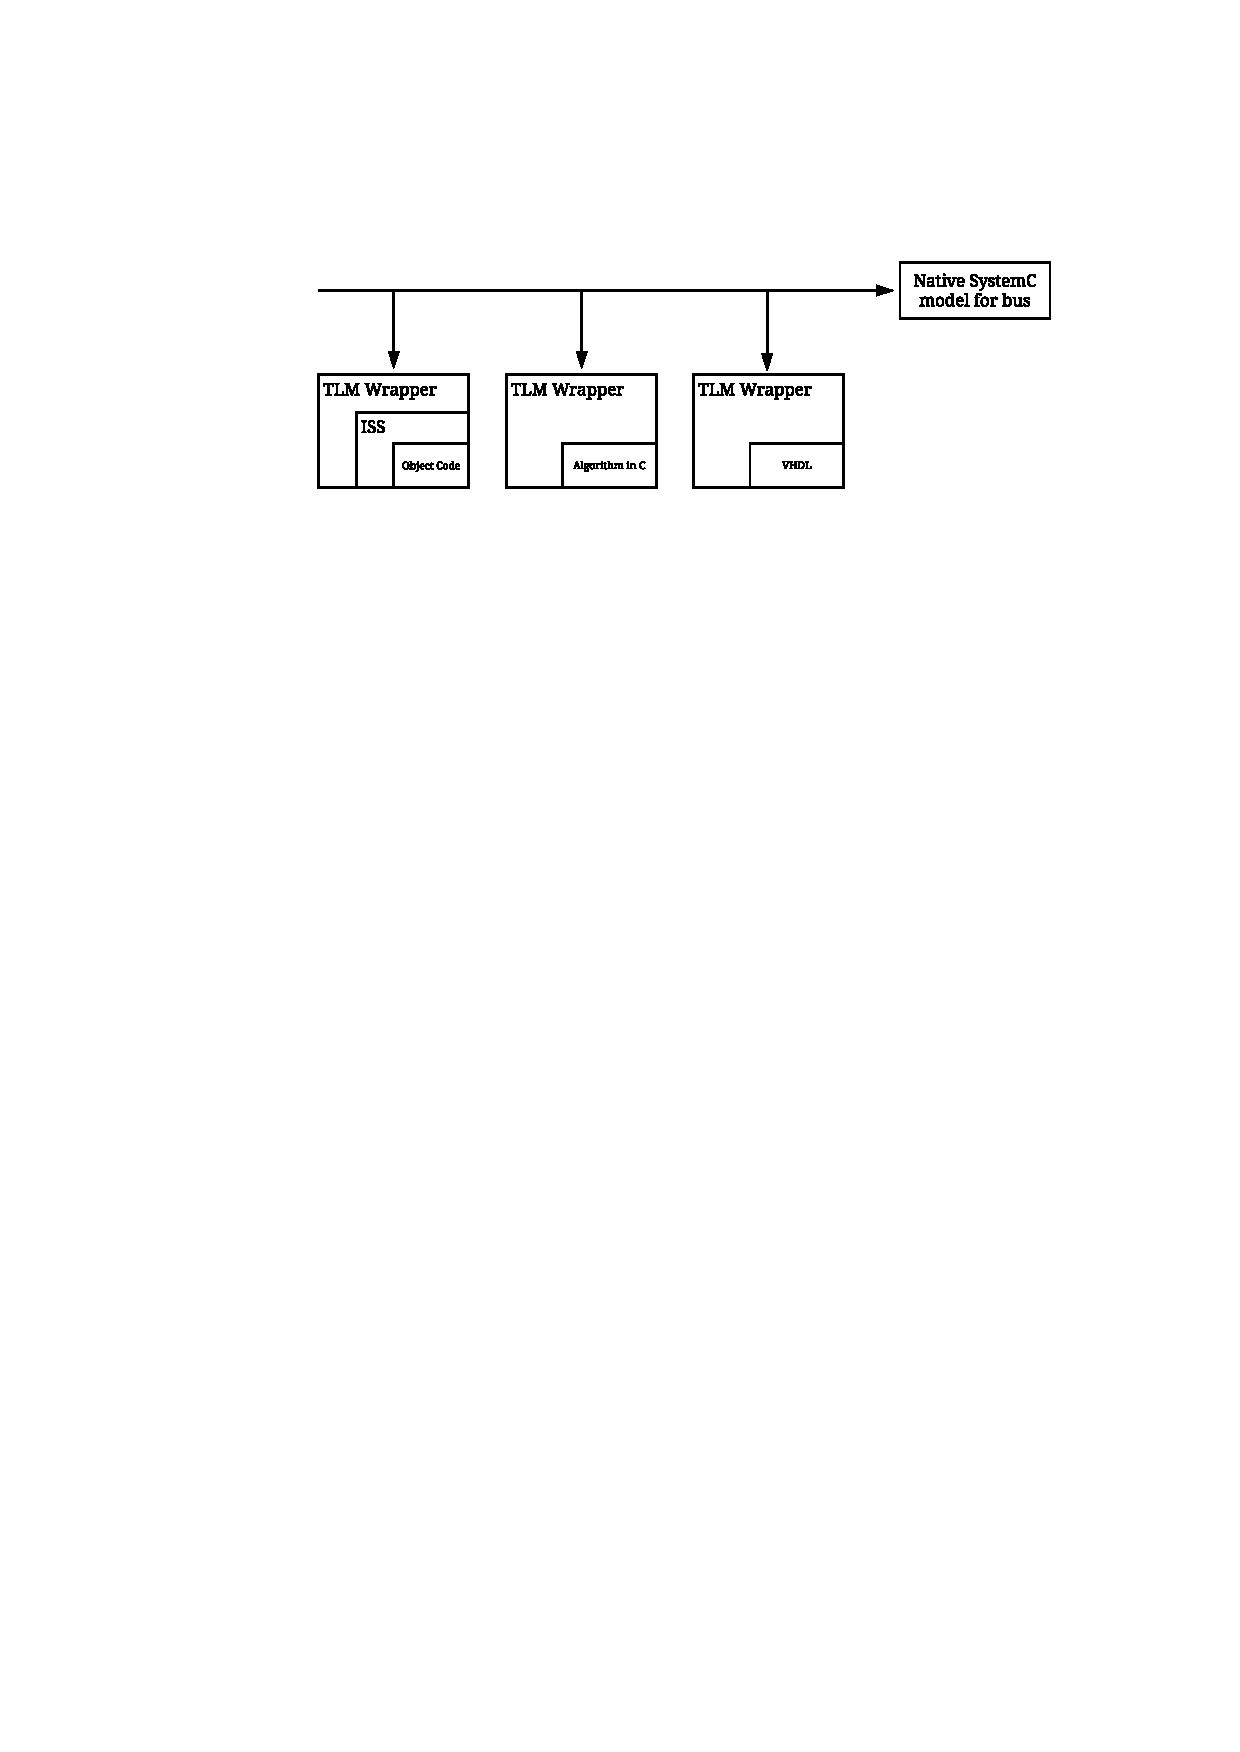
\includegraphics[width=.9\linewidth]{Figures/mixedSimulation.pdf}
\caption{\label{fig:org13715b0}
TLM 2.0 as a mixed language simulation technology}
\end{figure}

Modularity, or else IP block \textbf{interoperability}, is TLM's niche.
It enables the reuse of IP components in a "plug and play" fashion.
Having a library of verified IP blocks at his disposal, the engineer is able to create new virtual platforms fast and "effortlessly".
TLM is relevant at every interface where an IP block needs to be plugged into a bus.
TLM was designed with \textbf{memory-mapped} communication in mind.

To be suitable for productive software development, a virtual platform needs to be fast: it must be able to boot operating systems in seconds.
It also needs to be accurate enough such that, code developed using standard tools on the virtual platform, will run unmodified on real hardware \cite{Leupers2010}. 
Compared to a standard RTL simulation, a TLM achieves a significant speed up by replacing communication through pin-level events with a single function call.
The logic is quite simple: less events means less context switches between the simulation kernel and the application software.
This is exactly what makes simulations faster, but at the same time being TLM's major source of criticism.

\subsubsection{TLM 2.0 Terminology}
\label{sec:org1e385b1}
TLM 2.0 classifies IP blocks as initiator, target and interconnect components.
The terms initiator and target come forth as a replacement for the anachronistic terms master and slave.

An \textbf{initiator} is a component that initiates new transactions.
It is the initiator's duty to allocate memory for the payload.
Payloads are always passed by reference.

A \textbf{target} component acts as the end point of a transaction. 
As such, it is responsible for providing a response to the initiator.
Request and response are combined into a payload.
Thus, the target responds by modifying certain fields in the payload.

An \textbf{interconnect} component is responsible for routing a transaction on its way from initiator to target.
The route of a transaction is not predefined.
Routing is dynamic; it depends on the attributes of the payload, mainly its address field.
There is no limitation on the number of interconnect components participating in a transaction. 
An initiator can also be directly connected to a target.
Since an interconnect can be connected to multiple initiators and targets, it must be able to perform \textbf{arbitration} in case transactions "collide".

The role of a component is not statically defined and it is not limited to one.
It is determined on a transactions basis. 
For example, it may function as an interconnect component for some transactions, and as a target for other transactions.

Transactions are sent through initiator \textbf{sockets}, and received through target sockets.
Initiator sockets are used to forward method calls "up and out of" a component, while target sockets are used to allow method calls "down and into" a component.
It goes without saying that an initiator must have at least one initiator socket, a target at least one target socket and a interconnect must possess both.

All the above terms are illustrated in Figure \ref{fig:orgf1a2d0d}.
Each initiator-to-target socket connection supports both a forward and a backward path by which interface methods can be called in either direction.

\begin{figure}[htbp]
\centering
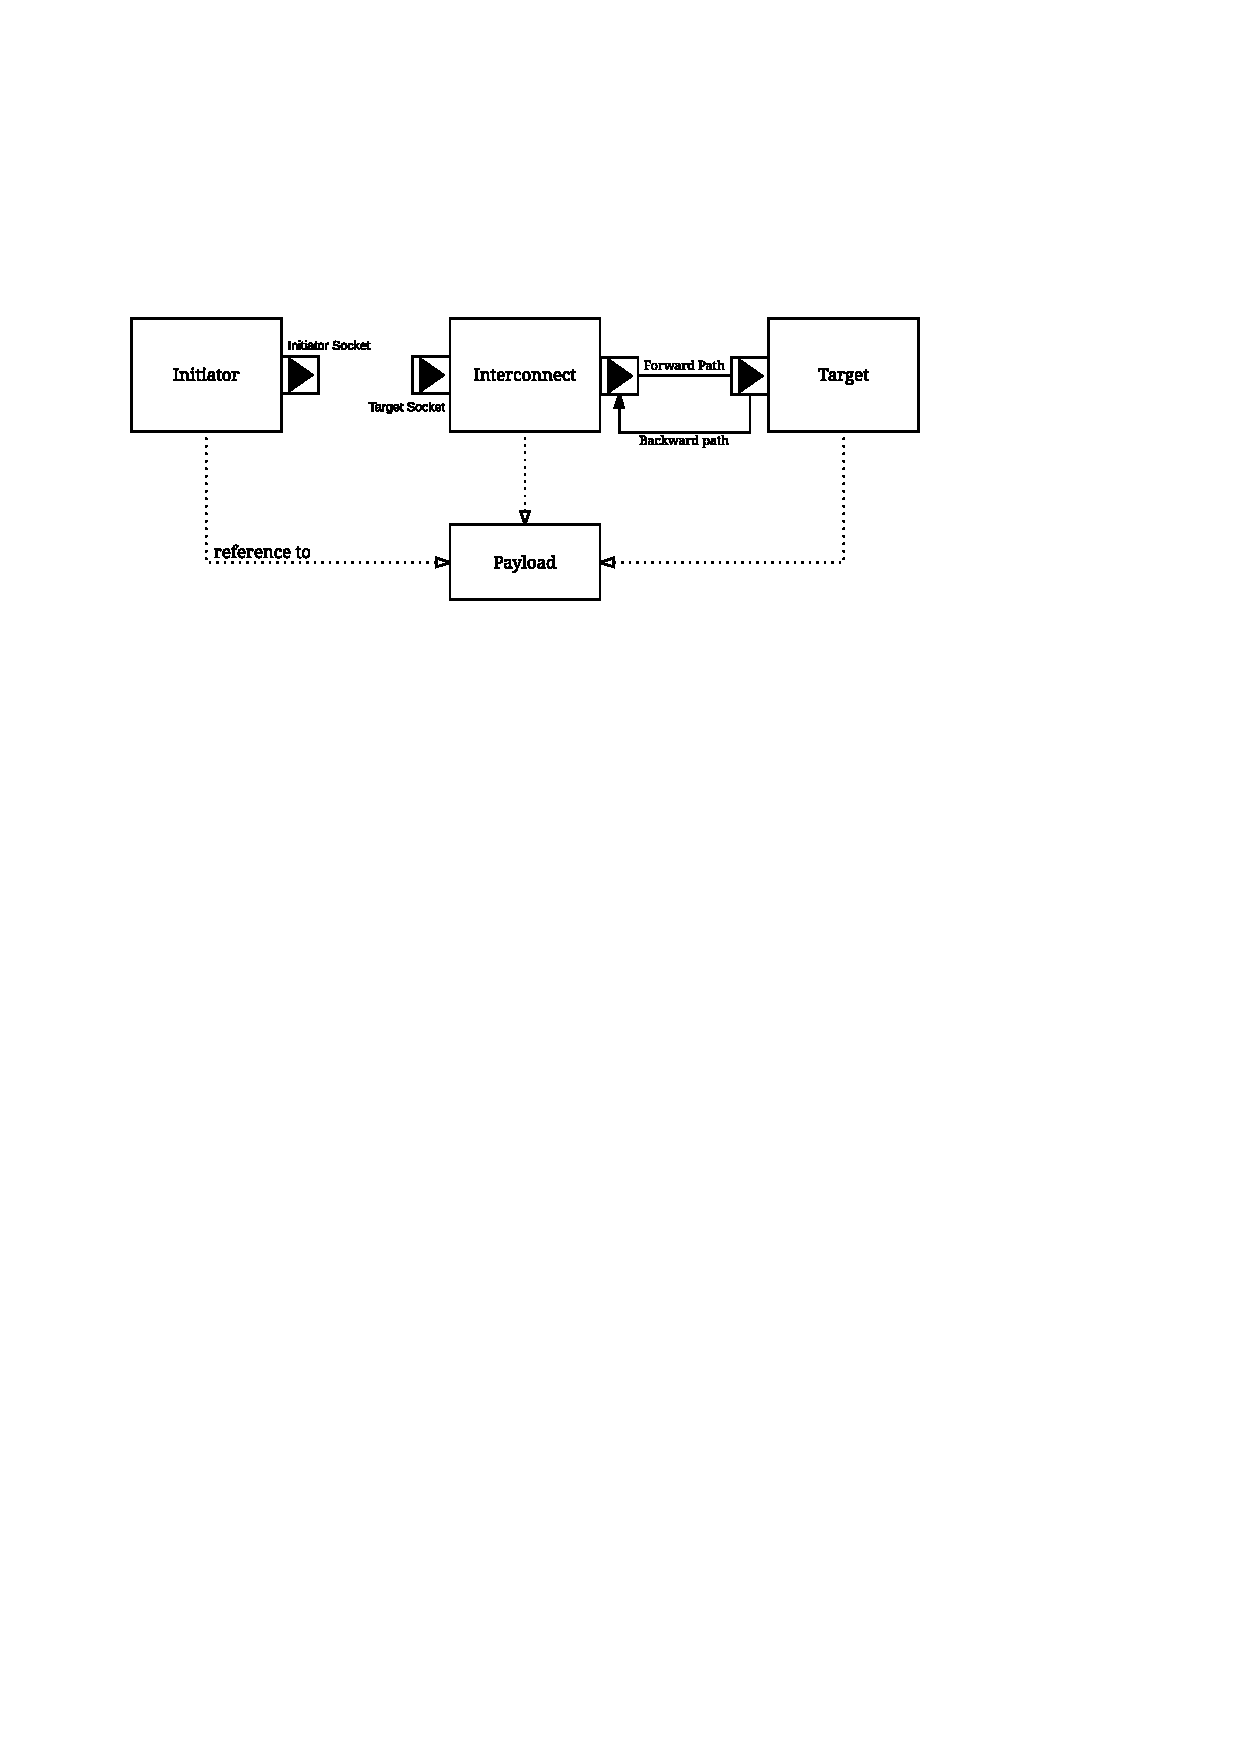
\includegraphics[width=.9\linewidth]{Figures/TLMterminology.pdf}
\caption{\label{fig:orgf1a2d0d}
TLM Sockets}
\end{figure}

\subsubsection{Generic Payload}
\label{sec:org9320766}
The basic argument that is passed, by reference, in communicative method calls is called the \textbf{payload}.
The choice of \texttt{tlm\_generic\_payload} as the type of the payload is a necessary condition for enabling interoperability between IP blocks from different vendors.
The \texttt{tlm\_generic\_payload} is a \textbf{structure} that encapsulates generic attributes relevant to a generic memory mapped bus communication.

The structure possesses an extensions mechanism, the designer can use to define more specific memory mapped bus architectures (e.g. ARM's AMBA).
An \textbf{interoperable} TLM 2.0 component must depend only on the generic attributes of the generic payload.
The presence of attributes through the extension mechanism can be ignored without breaking the functionality of the model.
In such a case, the extensions mechanism carries simulation metadata like pointers to module internal data structures or timestamps.

The following table lists all fields applicable on a \texttt{tlm\_generic\_payload}:

\begin{center}
\begin{tabular}{lll}
Attribute & Type & Modifiable by\\
\hline
Command & \texttt{tlm\_command} (enum) & Initiator only\\
Address & \texttt{uint64} & Interconnect only\\
Data pointer & \texttt{unsigned char*} & Initiator only\\
Data length & \texttt{unsigned int} & Initiator only\\
Byte enable pointer & \texttt{unsigned char*} & Initiator only\\
Byte enable length & \texttt{unsigned int} & Initiator only\\
Streaming width & \texttt{unsigned int} & Initiator only\\
DMI hint & \texttt{bool} & Any\\
Response status & \texttt{tlm\_response\_status} (enum) & Target only\\
Extensions & \texttt{(tlm\_extension\_base*)[]} & Any\\
\end{tabular}
\end{center}

\begin{itemize}
\item \textbf{Command:} Set to either \texttt{TLM\_READ} for read, \texttt{TLM\_WRITE} for write or \texttt{TLM\_IGNORE} to indicate that the command is set in the extensions mechanism.
\item \textbf{Address:} Can be modified by interconnects since by definition an interconnect must bridge different address spaces.
\item \textbf{Data pointer:} A pointer to the actual data being transferred.
\item \textbf{Data length:} Related to the data pointer, indicates the number of bytes that are being transferred.
\item \textbf{Byte enable pointer:} A pointer to a byte enable mask that can be applied on the data (0xFF for data byte enabled, 0x00 for disabled).
\item \textbf{Byte enable length:} Only relevant when the byte enable pointer is not null. If this number is less than the data length, the byte enable mask is applied repeatedly.
\item \textbf{Streaming width:} Must be greater than 0. If the data length \(\neq\) streaming width, then a streaming transaction is implied. Largest address defined by the transaction is (address + streaming width - 1), at which point the address wraps around.
\item \textbf{DMI hint:} A hint given to the initiator of whether he can bypass the transport interface and access a target's memory directly through a pointer.
\item \textbf{Response status:} The initiator must set it to \texttt{TLM\_INCOMPLETE\_RESPONSE} prior to initiating the transaction. The target will set it to an appropriate value indicating the outcome of the transaction. For example for a successful transaction the value is \texttt{TLM\_OK\_RESPONSE}
\item \textbf{Extensions:} The mechanism for allowing the generic payload to carry protocol specific attributes.
\end{itemize}

\subsubsection{Coding Styles and Transport Interfaces}
\label{sec:org2a4d607}
TLM defines two coding styles: the \textbf{Loosely-Timed} (LT) and the \textbf{Approximately-Timed} (AT).
Coding styles are not syntactically enforced: they are just guidelines that improve code readability.
LT is suited for describing virtual platforms intended for software development.
However, where additional timing accuracy is required, usually in architectural analysis, the AT style is employed.
Virtual platforms typically do not contain many cycle-accurate models of complex components because of the performance impact. 
The two coding styles are distinguished by the \textbf{transport interface} which components realize.
\subsubsection{The Loosely-Timed coding style}
\label{sec:org5d3b933}
The LT coding style uses the \textbf{blocking transport interface}, distinguished by the forward path method \texttt{b\_transport(PAYLOAD&, sc\_time&)}.
It is the simplest of the transport interfaces, in which each transaction is required to complete in a single interface method call.
The method, apart from the payload, takes a timing annotation argument.
Figure \ref{fig:sequence} demonstrates a possible interaction between components, during a blocking transport.
Typically, components execute transactions in the order in which they are received.
By definition, the blocking transport method may block, that is call \texttt{wait}, somewhere along the forward path from initiator to target.

\begin{figure}[htpb]
\centering
\includestandalone{./Figures/blocking_transport}
\caption{Loosely Timed coding style: Blocking interface sequence} 
\label{fig:sequence}
\end{figure}

The purpose of the timing annotation argument is to notify components that a particular transaction reaches them at \texttt{sc\_time\_stamp() + delay}.
The argument \texttt{delay} is the timing annotation argument, while \texttt{sc\_time\_stamp()} is a SystemC function that returns global simulation time.
Whether the semantics of the timing annotation argument are respected, is coding style dependent.
In the LT coding style the timing annotations may be disregarded.

In Figure \ref{fig:sequence} both interconnect and target only increment the timing annotation argument.
The initiator respects the timing annotation semantics and thus calls \texttt{wait(sc\_time)} once the transaction is completed.
Thus, the initiator will synchronize its local perception of time with global simulation time.
The existence of a local perception of time, different from global simulation time, is indicated by the non zero value of the timing annotation argument.

Appendix \ref{AppendixE} demonstrates the simplest TLM model that can be constructed: a system with one initiator (e.g. a processor) and one target (e.g. a memory).

\subsubsection{Temporal Decoupling}
\label{sec:org2cca2a8}
Figure \ref{fig:temporal_decoupling} illustrates the interaction between two LT initiators and one LT target component.
For the first two transactions of the simulation both Initiator1 and Target disregard the timing annotation, and run ahead of simulation time.
This phenomenon, which applies in the LT coding style, is called \textbf{temporal decoupling}.
It is evident by the increasing value of the timing annotation argument.
In the third transaction received, the target chooses to synchronize by calling \texttt{wait}.
As a result, Initiator2 will be scheduled for execution by the SystemC kernel.
After synchronization, notice that the target resets the timing annotation argument.

Temporal decoupling is exactly what makes LT simulations faster, by avoiding context switches between the SystemC kernel and initiator threads.
Synchronization with \texttt{wait} results in a context switch. 
In Figure \ref{fig:temporal_decoupling}, instead of having four context switches, one per transaction, there are only two.
However, temporal decoupling introduces causality hazards.
For example consider the second transaction issued by Initiator1 and the one issued by Initiator2.
If timing annotation semantics were respected, the execution order between these two transactions should have been the opposite.

\begin{figure}[htpb]
\centering
\includestandalone{./Figures/temporal_decoupling}
\caption{Temporal Decoupling with the Loosely-Timed coding style} 
\label{fig:temporal_decoupling}
\end{figure}

In order to avoid ad hoc synchronization logic in temporally decoupled components, TLM 2.0 provides a set of utilities for controlling it in a structured manner. 
These utilities are based on the concept of a \textbf{time quantum}.
The time quantum defines the maximum amount of time an initiator's local perception of time can be ahead of global simulation time.
Each initiator is responsible for checking its local time offset against the time quantum, and explicitly synchronize once the quantum has been exceeded.

The value of the quantum is user-defined, and the choice represents a trade-off between simulation speed and accuracy.
A small value gives high accuracy but limited speedup.
A large value gives the best speedup but also introduces more causality violations.
The use of the time quantum facilities is demonstrated in Appendix \ref{AppendixEB}.

A major concern, when implementing temporally decoupled target and interconnect components, is the \textbf{reentrancy} of the \texttt{b\_transport} interface method.
Reentrancy is about the safety of calling a function a multitude of times, before any previous invocation is completed.
For example, recursive functions must be reentrant or \textbf{pure}.
A pure function should not use any global or function-static variables.

To understand the need for reentrancy in the \texttt{b\_transport} method, consider the last two transactions in Figure \ref{fig:temporal_decoupling}.
The target's \texttt{b\_transport} method would is called again, in Initiator2's context , before the previous invocation (third transaction of Initiator1) is completed.

\subsubsection{Criticism}
\label{sec:org77b6859}
Some System level designers consider TLM 2.0 a step towards the wrong direction \cite{Liu2015}.
The major problem identified in TLM is the elimination of explicit channels, which were a key contribution in the early days of research on system-level design \cite{Liu2015}.
Communication in TLM looks like a remote function call \cite{Ecker2009}: a process, encapsulated in a module, executes a method of another module, in its own context.
The term \textbf{transaction} in TLM indicates exactly this remote function call, while the term \textbf{payload} indicates its most important argument.
The principle of "Separation of concerns between execution and communication" has been abandoned; execution obfuscates communication.
The RISC project (see Section \ref{sec:orge7b4ee6}) has not (yet) supported the TLM API for this exact reason.

The need for \textbf{recoding} SystemC TLM 2.0 models, in order to allow parallel execution, has manifested. 
Recoding must reconstitute the separation of concerns between computation and communication.
As a result, TLM could serve the following purposes:
\begin{itemize}
\item A front end language, due to its simplicity
\item A sequential option for "smaller" models, since parallelism may add a significant execution overhead.
\end{itemize}

Finally, we would also like to note the absence of any built-in functionality to abort simulation when causality has been violated.
\clearpage

\subsection{Message Passing Interface}
\label{sec:org12eae92}
In any Message Passing Interface, the concept of communication is modeled as message passing.
The DE MoC concept of an event is associated with either a message transmission or a message reception statement.
This fact must be emphasized: an event is not a message, it is not something to be exchanged.
It is rather the exchange of a message that yields two events.
The DE MoC concept of a process can be reduced to an instance of a computer program that is being executed \cite{Tanenbaum1998} in an Operating System's (OS) environment.

Section \ref{sec:org0eaab05} presents the rationale behind choosing MPI, as the means for achieving spacial decomposition, in the proposed OoO PDES.
In section \ref{sec:org0ff3938} and \ref{sec:orgd81ee2c} we present the semantics of the Message Passing Interface (MPI) communication primitives.

This unit is complemented by Appendix \ref{AppendixD}, where the reader can experience MPI's elegance, by means of an example implementation of the pipeline pattern.

\subsubsection{Rationale}
\label{sec:org0eaab05}
\textbf{Message Passing Interface} 3.0 (MPI) \cite{MessagePassingInterfaceForum2012} was the preferred implementation framework for the proposed OoO PDES.
The rationale behind this choice can be summarized as follows:
\begin{itemize}
\item The ease of expressing process communication, that leads to improved readability and maintainability, when compared to other process manipulation APIs (e.g. POSIX)
\item Scalability. Any computing device or cluster with Internet Access, from a Raspberry Pi to Tianhe-2, can participate in the simulation.
If the MPI runtime environment is configured properly, the software developer may remain agnostic about the exact communication fabric (e.g. shared memory, TCP/IP, DAPL).
\item High performance. Prior to version 3.0, MPI was deemed a bad choice for applications confined in shared memory nodes. 
Threading APIs (e.g. OpenMP), or hybrid approached were a more favorable choice.   
With the introduction of MPI 3.0, shared memory regions, for conducting communication apart from message passing, can be exposed to processes.
\end{itemize}

\subsubsection{Semantics of point-to-point Communication in MPI}
\label{sec:org0ff3938}
MPI is a message passing library interface specification, standardized and maintained by the Message Passing Interface Forum.
It is currently available for C/C++, FORTRAN and Java from multiple vendors (Intel, IBM, OpenMPI).
MPI addresses primarily the message passing parallel programming model, 
in which data is moved from the address space of one process to that of another process through cooperative operations on each process \cite{MessagePassingInterfaceForum2012}.

The basic communication primitives are the functions \texttt{MPI\_Send(...)} and \texttt{MPI\_Recv(...)}.
Their arguments specify, among others things, a data buffer and the peer process' or processes' unique id assigned by the MPI runtime.
By default, message reception is blocking, while message transmission may or may not block.
One can think of message transfer as consisting of the following three phases
\begin{enumerate}
\item Data is pulled out of the send buffer and a message is assembled
\item A message is transferred from sender to receiver
\item Data is pulled from the incoming message and disassembled into the receive buffer
\end{enumerate}

\textbf{Order:}
Messages are non-overtaking.
If a sender sends two messages in succession to the same destination, 
and both match the same receive (a call to \texttt{MPI\_Recv}), 
then this operation cannot receive the second message if the first one is still pending. 
If a receiver posts two receives in succession,
and both match the same message, 
then the second receive operation cannot be satisfied by this message, if the first one is still pending. 
This requirement facilitates matching of sends to receives and also guarantees that message passing code is deterministic.

\textbf{Fairness:}
MPI makes no guarantee of fairness in the handling of communication. 
Suppose that a send is posted. 
Then it is possible that the destination process repeatedly posts a receive that matches this send, 
yet the message is never received, 
because it is each time overtaken by another message, 
sent from another source. 
It is the programmer’s responsibility to prevent starvation in such situations.


\subsubsection{MPI Communication Modes}
\label{sec:orgd81ee2c}
The MPI API contains a number of variants, or \textbf{modes}, for the basic communication primitives.
They are distinguished by a single letter prefix (e.g. \texttt{MPI\_Isend(...)}, \texttt{MPI\_Irecv(...)}).
As dictated by the MPI version 3.0, the following communication modes are supported \cite{MessagePassingInterfaceForum2012}:

\textbf{No-prefix for standard mode: \texttt{MPI\_Send(...)}}
In this mode, it is up to MPI to decide whether outgoing messages will be buffered. 
MPI may buffer outgoing messages. 
In such a case, the send call may complete before a matching receive is invoked. 
On the other hand, buffer space may be unavailable, or MPI may choose not to buffer outgoing messages, for performance reasons. 
In this case, the send call will not complete, blocking the transmitting process, until a matching receive has been posted, and the data has been moved to the receiver.

\textbf{B for buffered mode: \texttt{MPI\_Bsend(...)}} 
A buffered mode send operation can be started whether or not a matching receive has been posted. 
It may complete before a matching receive is posted. 
However, unlike the standard send, this operation is local, and its completion does not depend on the occurrence of a matching receive. 
Thus, if a send is executed and no matching receive is posted, then MPI must buffer the outgoing message, so as to allow the send call to complete. 
A buffered send operation that cannot complete because of a lack of buffer space is erroneous. 
When such a situation is detected, an error is signaled that may cause the program to terminate abnormally. 
On the other hand, a standard send operation that cannot complete because of lack of buffer space will merely block, 
waiting for buffer space to become available or for a matching receive to be posted. 
This behavior is preferable in many situations. 
Consider a situation where a producer repeatedly produces new values and sends them to a consumer. 
Assume that the producer produces new values faster than the consumer can consume them. 
If buffered sends are used, then a buffer overflow will eventually occur. 
Additional synchronization has to be added to the program so as to prevent this from occurring. 

\textbf{S for synchronous mode: \texttt{MPI\_Ssend(...)}}
A send that uses the synchronous mode can be started whether or not a matching receive was posted. 
However, the send will complete successfully only if a matching receive is posted, and the receive operation has started to receive the message sent by the synchronous send.
Thus, the completion of a synchronous send not only indicates that the send buffer can be reused, 
but it also indicates that the receiver has reached a certain point in its execution, 
namely that it has started executing the matching receive. 
If both sends and receives are blocking operations then the use of the synchronous mode provides synchronous communication semantics: 
a communication does not complete at either end before both processes \textbf{rendezvous} at the communication point.

\textbf{R for ready mode: \texttt{MPI\_Rsend(...)}}
A send that uses the ready communication mode may be started only if the matching receive is already posted. 
Otherwise, the operation is erroneous and its outcome is undefined.
Ready sends are an optimization when it can be guaranteed that a matching receive has already been posted at the destination.
On some systems, this allows the removal of a hand-shake operation that is otherwise required and results in improved performance. 
A send operation that uses the ready mode has the same semantics as a standard send operation, or a synchronous send operation; 
it is merely that the sender provides additional information to the system (namely that a matching receive is already posted), that can save some overhead. 

\textbf{I for non-blocking mode: \texttt{MPI\_Isend(...)}, \texttt{MPI\_Ibsend(...)}, \texttt{MPI\_Issend(...)} and \texttt{MPI\_Irecv(...)}}
Non-blocking message passing calls return control immediately (hence the prefix I), 
but it is the user's responsibility to ensure that communication is complete, 
before modifying/using the content of the data buffer.
It is a complementary communication mode that works en tandem with all the previous.
The MPI API contains special functions for testing whether a communication is complete, or even explicitly waiting until it is finished.
In Appendix \ref{AppendixD} the reader can find an example use case for this communication mode.


\clearpage

\section{Out of Order PDES with MPI}
\label{sec:orgb236fc3}
In Section \ref{sec:org9d36a74} and \ref{sec:org3bb5bd9} we present the conservative synchronization algorithm known as \textbf{Chandy Misra Bryantt} (CMB).
In Section \ref{sec:org7e0e641} a pseudocode description of the CMB is demonstrated. The pseudocode incorporates MPI communication primitives.

\subsection{The Chandy/Misra/Bryant synchronization algorithm}
\label{sec:org9d36a74}
The synchronization algorithm at the heart of the proposed OoO PDES is known as the \textbf{Chandy/Misra/Bryant (CMB)} \cite{Bryant} \cite{Chandy1979}.
Historically, it has been the first of the family of conservative synchronization algorithms \cite{Fujimoto1990}.
According to the algorithm, the physical system to be simulated must be modeled as a number of communicating sequential processes.
The system's state, a set of variables, is partitioned amongst the system's processes.
Execution is reactive; it is initiated by an event and produces further events and side-effects (changes in the system's state variables).
Each process keeps its own perspective of logic time through a counter.
The counter advances according to the timestamp of the last event selected for execution.

Based on the system's state segregation, a static determination of which processes are interdependent can be established.
This is indicated by placing a \textbf{link} for each pair of dependent processes.
From a process' perspective a link can be either outgoing, meaning that events are sent via the link, or incoming, meaning that events are received through it.
An incoming link must encapsulate an unbounded \footnote{The system description is quite similar to that of another MoC called \textit{"Kahn process networks"} \cite{Editor2014}, which also uses unbounded FIFOs as a channel communication mechanism.
The difference is qualitative: the DE MoC incorporates timing semantics.
A Kahn process network is \textbf{untimed} by definition.} First-In First-Out (FIFO) data structure  for storing incoming events, in the order they are received.

The order by which events are received is \textbf{chronological}; non decreasing timestamp order.
This system-wide property is maintained by making each process select for computation the event that has the smallest timestamp.
A formal proof of how this local property \textbf{induces} a system-wide property can be found in \cite{Bryant} \cite{Chandy1979}.

Chronological reception of events is a necessary, but not sufficient, condition for ensuring \textbf{causality}.
The algorithm deals with the "is an event safe to execute" dilemma by \textbf{blocking} a process until each of its incoming links contains an event.
All the above are demonstrated in Algorithm \ref{alg:initial_CMB}. 
The synchronization algorithm is realized as a process' main event loop.

\begin{LATEX}
\begin{algorithm}
\caption{Process event loop, without deadlock avoidance}
\label{alg:initial_CMB}
\begin{algorithmic}[1]

   \While{process time < some T}  
      \State \textbf{Block} until each incoming link contains at least one event
      \State select event M, with the \textbf{smallest} timestamp across all incoming links.
      \State set process' \textbf{counter} = timestamp(M)
      \State \textbf{execute} event M
      \State \textbf{communicate} resulting events over the appropriate links
   \EndWhile

\end{algorithmic}
\end{algorithm}
\end{LATEX}

\subsection{Deadlock Avoidance}
\label{sec:org3bb5bd9}
The naive realization of the process' event loop presented in Algorithm \ref{alg:initial_CMB} leads to deadlock situations, like the one depicted in Figure \ref{fig:org9269447}.
The links placed along the outer loop are empty (dashed lines), thus simulation has halted, even though there are pending events (across the links of the inner loop).

A global simulation moderator could easily detect deadlocks and allow the process, that has access to the event with the global minimum timestamp, to resume execution.
The presence of a moderator, however, would violate the distributed nature of the simulation, and thus increase the implementation complexity of the simulation environment.
For the context of this thesis, a distributed mechanism is more favorable.
What follows is the presentation of a distributed mechanism for overcoming these situations, referred to as the \textbf{null-event deadlock avoidance} \cite{Fujimoto1999}.

\begin{figure}[htbp]
\centering
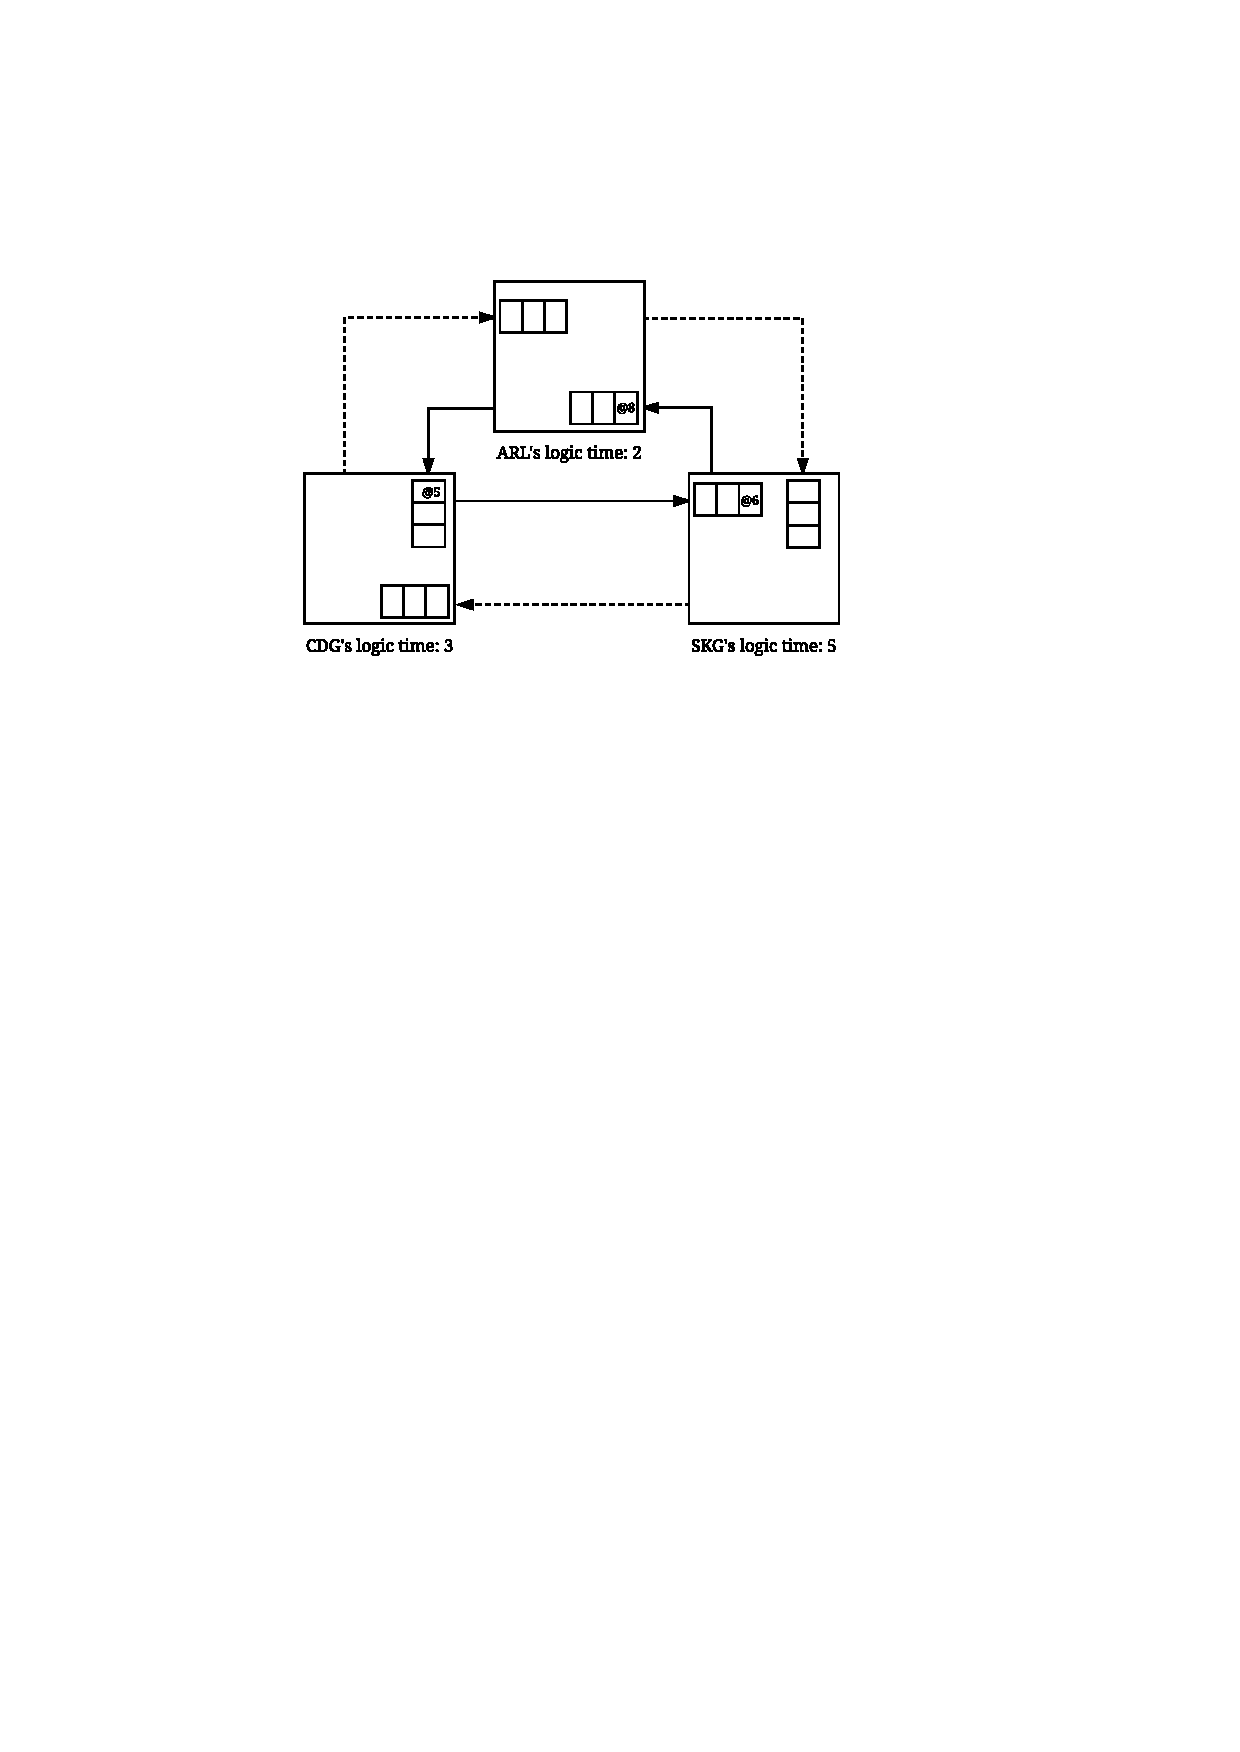
\includegraphics[width=0.64\linewidth]{Figures/deadlockScenario.pdf}
\caption{\label{fig:org9269447}
Deadlock scenario justifying the use of Null messages in the CMB}
\end{figure}

Figure \ref{fig:org9269447} demonstrates an air traffic simulation, where the airports (ARL, CDG and SKG) constitute the simulation processes.
The events exchanged between the airports represent flights (the time unit being arbitrary).
Furthermore, it is assumed that there is an \textbf{a priori} knowledge concerning the flight time between airports.
This knowledge is referred to as the \textbf{lookahead} and takes the form of a function \((P \times P) \rightarrow \mathbb{N}\).
By selecting the distance between every airport to be 3 time units, one can deduce the following:
If SKG is at time 5, then ARL or CDG should not expect any flight arriving from SKG before time 8.

The simulation is deadlocked: all of the airports contain an empty link and therefore, according to Algorithm \ref{alg:initial_CMB}, they must block.
At deadlock, the counter values for each airport are: (ARL,2), (SKG,5), (CDG,3).
The intuition behind any technique, that could break the deadlock, should rely on the following observation:
if CDG knew that SKG is at time 5, then it could be able to accept the incoming flight from ARL, without breaking causality.

To "communicate" this information, SKG could create a special kind of event, a \textbf{null event} that does not represent a flight. 
Its timestamp should be 8 (counter+lookahead) and the event should be placed on all of SKG's outgoing links.
With this null event, SKG is informing the other airports about its time perspective.
A null event is still an event, so CDG would acknowledge it during the selection phase, and thus would be able to receive the flight from ARL.
CDG now sits at 5 and in the same fashion it could broadcast a null event with timestamp 8, that would in turn unblock ARL.
It is evident that the deadlock situation has been resolved, at the expense of flooding the communication links with null events.

The modified, for deadlock avoidance, algorithm is described in Algorithm \ref{alg:null-event}.
The important facts one must keep in mind with this deadlock avoidance mechanism are:
\begin{itemize}
\item The logic time counter of a process is still determined by the last event selected for execution.
\item Null events are created when a process updates its logic time counter.
\item Each process propagates null events on all of its outgoing links.
\item The efficiency of this mechanism is highly dependent on the designer's ability to determine sufficiently large lookaheads.
\end{itemize}

\begin{LATEX}
\begin{algorithm}
\caption{Process event loop, with deadlock avoidance}
\label{alg:null-event}
\begin{algorithmic}[1]

   \While{process clock < some T}  
      \State \textbf{Block} until each incoming link FIFO contains at least one event
      \State Remove event M with the smallest timestamp from its FIFO.
      \State Set process' clock = timestamp(M)
      \State \textbf{React} to event M
      \State \textbf{Communicate} either a null or meaningful event to each outgoing link with timestamp = clock + lookahead
   \EndWhile

\end{algorithmic}
\end{algorithm}
\end{LATEX}

\subsection{MPI Realization of CMB}
\label{sec:org7e0e641}
Listing \ref{alg:CMB_mpi} is a pseudo code, sketching out the CMB synchronization algorithm with null event deadlock avoidance, using MPI's communication primitives.
The mechanism should be incorporated in a process' main event loop.
It is quite obvious that the concept of an event has been reduced to a simple data structure, with the timestamp being the most important field.
Much like SystemC, logic time modeling is an implied vector \((t,n,l)\): \(t\) is the value of a process' counter, \(n\) (delta) and \(l\) are implied by, the event's position in the links' FIFO and the process' rank, respectively.
\begin{LATEX}
\begin{algorithm}
\caption{CMB Process event loop in MPI}
\label{alg:CMB_mpi}
\begin{algorithmic}[2]

   \While{process clock < some T}  
      \State post a \texttt{MPI\_Irecv} on each incoming peer process
      \State post a MPI\_Wait: block until every receive has been completed
      \State save each message received in a separate, per incoming link, FIFO.
      \State identify message M with the smallest timestamp
      \State set counter = timestamp(M)
      \State process message M
      \State post a \texttt{MPI\_Issend} to each outgoing link with timestamp = counter + Lookahead(myRank, recvRank)
   \EndWhile

\end{algorithmic}
\end{algorithm}
\end{LATEX}


\clearpage

\section{Methodology}
\label{sec:org1d9dc6c}
This chapter is a synoptic presentation \footnote{The source code for the case studies is publicly accessible in the following github repository: \url{https://github.com/kromancer/Thesis}.} of the case studies constructed for the evaluation of the proposed OoO PDES.
All necessary simulations were carried out in a server equipped with two Intel Xeon E5-2603V3 processors, with a total of 128 GB of DDR4-1600 RAM.

Section \ref{sec:org527f491} presents an airtraffic simulation, following the example presented in Section \ref{sec:org3bb5bd9}.
The simulation incorporates a validation procedure: Causality hazards are detected and lead to simulation termination.
The Section is complemented with Appendix \ref{AppendixC}.
Section \ref{sec:org7189b0e} presents the simulation of a cache-coherent multiprocessor.
For this case study 2 models where constructed: A Loosely-Timed SystemC TLM 2.0 model, simulated by SystemC's DES, 
and a "manually compiled" translation of it, compatible with the proposed OoO PDES.

\subsection{Case Study 1: Airtraffic Simulation}
\label{sec:org527f491}
The simulation is parameterized on the number of airports, their topological arrangement and each airport's flight schedule.
The \textbf{topological arrangement} of the airports is determined at compile time.
For example, the three airport topology described in Figure \ref{fig:org9269447} is demonstrated in Appendix \ref{AppendixC}

Figure \ref{fig:val} demonstrates the validation procedure for the simulation.
The following measures are taken to ensure correctness and remove bias:
\begin{itemize}
\item In a pre simulation step, a randomized \textbf{global flight schedule} is created.
Based on a flight's source field, the schedule is then distributed to the airports.
\item Prior to segregation, the global schedule is also "simulated" sequentially. 
The sequential "simulation" is quite trivial and does not require a DES:
The global schedule is traversed, and for every event a departure log entry and an arrival log entry are created.
The entries are sorted and stored in the \textbf{reference global log}.
\item During simulation, airports exchange messages indicating flights, and every airport is responsible for creating a \textbf{log} of departures and arrivals.
The logs are saved as .csv files for post simulation inspection.
From an airport's perspective, its \textbf{flight schedule} is modeled as an incoming link, which is filled upon instantiation.
The system's computational objective is to create a \textbf{global log} of departures/arrivals.
The global log is consolidated post parallel simulation.
\item An airport can detect a \textbf{causality hazard} by simply checking if its counter (its perspective of logic time) is about to become less than its current value.
When causality hazards are detected, a process aborts simulation.
\item Finally, the global log is checked against the reference global log for completeness.
\end{itemize}

\begin{figure}[htpb]
\centering
\tikzstyle{block} = [draw, fill=white, rectangle]

\begin{tikzpicture}[node distance=2cm, block/.style={ rectangle, draw=black, thick, fill=white, text centered, rounded corners, minimum height=2em }]
    \node [anchor=south,block, text width=6.3cm]                      (n1)   {\scriptsize Generate randomized global flight schedule};
    \node [anchor=south,block, below left of=n1, text width=4.3cm]    (n2)   {\scriptsize Segragate per airport \\ e.g. \texttt{fligth\_schedule\_ARL.csv}};
    \node [anchor=south,block, below of=n2, text width=4.3cm]         (n3)   {\scriptsize OoO PDES \\ Causality hazard $\rightarrow$ \texttt{MPI\_ABORT}};
    \node [anchor=south,block, below of=n3, text width=4.3cm]         (n5)   {\scriptsize Consolidate \& order logs};
    \node [block, right=0.6cm of n3, text width=1.3cm]                  (n4)   {\scriptsize Simulate Serially };
    \node [block, below of=n5] (n6) {\scriptsize Compare Logs};

    \draw[draw,->]       (n2|-n1.south) --  (n2.north);
    \draw[->]            (n2) --  (n3);
    \draw[->]            (n4|-n1.south) -- (n4.north);
    \draw[->]            (n3) --  (n5);
    \draw[->]            (n5) --  (n6);
    \draw[->]            (n4.south) |-  (n6.east);

\end{tikzpicture}
\caption{Case Study 1: Validation Procedure} 
\label{fig:val}
\end{figure}

The implementation is structured upon three C++ classes: \texttt{Process}, \texttt{Links} and \texttt{Flight}. 
Their relationship is quite simple: a \texttt{Process} "has a" \texttt{Links} and a \texttt{Links} "has many" \texttt{Flight}.
The class \texttt{Links} realizes a process' incoming links.
Outgoing links are realized implicitly: 
\begin{itemize}
\item The system's topology is deserialized by MPI, in the form  of \textbf{distributed-graph group communicators} \cite{MessagePassingInterfaceForum2012}, as demonstrated in Appendix \ref{AppendixC}.
Each process gets a communicator that represents its neighborhood, that is other processes that send and receive messages to/from this process.
\item The series of communication primitives used in Algorithm \ref{alg:CMB_mpi} have almost the same aggregate effect as the collective communication primitive \texttt{MPI\_Neighbor\_Allgather}.
With this collective communication primitive, the process sends the same message to all of its outgoing neighbors, and receives a (different) message from every incoming neighbor.
\item The communication will only block the process if either a message has not been received from every incoming neighbor, or the MPI runtime can not buffer the outgoing message.
The fact that outgoing messages can be buffered must be emphasized. 
This communication primitive is not synchronous, it does not denote a rendezvous point (see Section \ref{sec:orgd81ee2c}).
Moreover, it is now evident why outgoing links are realized implicitly: a process relies on MPI's buffering capabilities.
\item By employing this collective operation, communication and execution confront to the their simple definition, presented in Section \ref{sec:org409ed59}, where both input and output require/produce one event.
Furthermore, the implementation of the null-event deadlock avoidance mechanism becomes simple: a null-event occurs when a process receives a message that was not meant for it, that is the destination field of the flight does not match its own airport identity.
\end{itemize}
An airport's main event loop, the "hotspot" of \texttt{Process::run()}, is demonstrated in Figure \ref{fig:airport}.

\begin{figure}[htpb]
\centering
\begin{tikzpicture} [
    auto,
    decision/.style = { diamond, draw=black, thick, fill=white,
                        text badly centered,
                        inner sep=1pt, rounded corners },
    block/.style    = { rectangle, draw=black, thick, 
                        fill=white, text centered,
                        rounded corners, minimum height=2em },
    line/.style     = { draw, thick, ->, shorten >=2pt },
  ]
  % Define nodes in a matrix
  \matrix [column sep=5mm, row sep=5mm] {
                    & \node [decision] (n0) {\scriptsize\texttt{!readyToTerminate}};  & \\
                    & \node [block, text centered] (n1) {\small\texttt{MPI\_Neighbor\_Allgather(...)}}; & \\
                    & \node [block, text centered, text width=5.2cm] (n2) {\small\texttt{Flight e = links.nextFlight()} \small\texttt{counter = e.tstamp()}};    & \\
                    & \node [decision] (n3) {\scriptsize\texttt{!e.isOutbound()}};  & \node [block, text width=2.5cm] (n4) {\small\texttt{updateLog()} \texttt{sendbuf = e}}; & \\
                    & \node [decision] (n5) {\scriptsize\texttt{!e.isInbound()}};   & \node [block] (n6) {\small\texttt{updateLog()}}; & \\
                    & \node  (n7) {};   &  \node (n8) {};& \\
                    & \node [decision, text width=2.8cm] (n9) {\scriptsize\texttt{links.isAnyEmpty()} \small\texttt{||} \scriptsize\texttt{!e.isOutbound()}};  & \\
  };
  % connect all nodes defined above
  \begin{scope} [every path/.style=line]
    \path (n0)        --    (n1);
    \path (n1)        --    (n2);
    \path (n2)        --    (n3);
    \path (n3)        --    node [near start] {yes} (n4);
    \path (n4)        --++ (2,0) |-    (n8);
    \path (n3)        --    (n5);
    \path (n5)        --    node [near start] {yes} (n6);
    \path (n6)        --    (n8);
    \path (n5)        --    (n7);
    \path (n8)        --    (n7);
    \path (n7)        --    (n9);
    \path (n9)        --++ (-5,0) |-   node [near end] {yes}(n0);
    \path (n9)        --++ (-5,0) |-   node [near end] {no} (n2);
  \end{scope}
\end{tikzpicture}
\caption{Case Study 1: Airport's event loop} 
\label{fig:airport}
\end{figure}


\clearpage

\subsection{Case Study 2: Cache-coherent Multiprocessor}
\label{sec:org7189b0e}
A SystemC TLM 2.0 diagram of the cache-coherent multiprocessor that will be modeled can be found in Figure \ref{fig:org598f69a}.
Every component was coded in C++.
The processors are executing a "pseudoprogram": they are just generating memory accesses, based on a previously performed memory trace collection of an actual program.
The actual program was multithreaded (4 threads), and was experiencing (deliberately) the phenomenon known as "false sharing" \cite{Hennessy2011}.
The L1 Data caches are 8-way set associative, their size being parameterizable.
Coherence amongst the caches is realized through a Modified Shared Invalid (MSI) scheme, by a directory which acts like an inclusive L2 cache.
Since actual data are not needed, main memory presence is implied by the directory.

\url{Figures/multiprocessor.pdfno}







\clearpage

\section{Analysis}
\label{sec:org1cdc1b0}
Sections \ref{sec:orgbb0cec4} and \ref{sec:org5dbd9db} are related to the analysis of the first case study.
Section \ref{sec:org8a3fd73} discusses the most important aspect of the second case study: the transformation of a SystemC Loosely-Timed TLM 2.0 model to a model for the proposed OoO PDES.

\subsection{Time Complexity}
\label{sec:orgbb0cec4}
The following assumption is made: the time complexity of a deterministic DES (Section \ref{sec:org6436102}), is of the form \(\mathcal{O}(f(|\mathds{E}|))\).
In the proposed OoO PDES:

\begin{LATEX}
\begin{equation} 
   |\mathdbs(E)| = f(|\mathbb{P}|, \min\{lookahead(P_i,P_j)\}_{i,j \leq |\mathbb{P}|}).
\end{equation}
\end{LATEX}

In simpler terms: 
\begin{itemize}
\item The total number of simulation events is highly sensitive to the number of null messages.
\item The number of null messages produced is proportional to the minimum lookahead value across the system.
\item In the worst case, the minimum lookahead will be 1. This introduces a qualitative shift in time complexity, which now becomes: 
\(\mathcal{O}(f(t_{end}-t_{start}))\) with \(t_{end}\) and \(t_{start}\) being the timestamps of the first and last simulation events.
\end{itemize}
This well established empirical observation \cite{Fujimoto1999} for simulators dependent on the CMB algorithm, has been confirmed.

\subsection{Monotonicity of Communication}
\label{sec:org5dbd9db}
In the DE MoC, any communication function possessing the property \(e_1 \sqsubset e_2 \implies g(e_1) \sqsubset g(e_2)\) is called \textbf{monotonic}.
In the context of the proposed PDES, it can be easily proven that any communication function, that uses a constant lookahead per pair of processes, is monotonic.
The communication functions that are used in the case studies are monotonic.

And here comes a reasonable question: What happens if the lookahead function is not only influenced by \((P_i, P_j)\).
For example, consider the following situation: 
at an airport, an airplane's departure is followed by the departure of a faster airplane.
Both the flights are destined for the same target airport.
The faster aircraft is meant to arrive at the target airport sooner.
Using the visual understanding of the DE MoC from Section \ref{sec:org3dada3c}, the situation is captured in Figure \ref{fig:nonmon}.

\begin{figure}[htpb]
\centering
\begin{tikzpicture}[
arrow/.style={draw,->,>=stealth},
point/.style={circle,fill=black},
every node/.style={node distance = 10},
]
\node (p1) at (0,2) {$p_1$};
\node (p2) at (0,1) {$p_2$};
\node (p1l) at (0.2,2) {};
\node (p2l) at (0.2,1) {};
\node (p1r) at (8,2) {};
\node (p2r) at (8,1) {};

\draw[arrow] (p1l.center) to (p1r);
\path[arrow] (p2l.center) to (p2r);
\path[draw]  (p1l.center) edge (p2l.center);

\node[point, label={\small slow dep.}] (a) at (3,2) {};
\node[point, label={\small fast dep.}] (b) at (5,2) {};
\node[point, label=below:{\small fast arr.}] (c) at (2,1) {};
\node[point, label=below:{\small slow arr.}] (d) at (6,1) {};

%\node[point] (k) at (4,1) {};
%\node [below of = k] {a};
%\node[point, label=b] (l) at (7,2) {};

\path[arrow] (b) edge node [right] {} (c);
\path[arrow] (a) edge node [right] {} (d);
%\path[arrow] (k) edge node [right] {} (l);

\end{tikzpicture}
\caption{Non-monotonic communication in the DE MoC} 
\label{fig:nonmon}
\end{figure}

How can a DES cope with non-monotonic communication?
A naive approach would be to define a static execution schedule: first \(p_1\) and then \(p_2\).
The naivety of the approach lies in the following self-contradiction: why run a simulation if you already know its outcome?

The proposed PDES can not handle such a situation. 
Timestamps in \(p_2\) 's incoming link are not placed in an increasing timestamp order by \(p_1\) and thus \(p_1\) is bound to face a causality error: its local time will advance backwards.
It is therefore evident that the only way to tackle this situation, while keeping the CMB synchronization mechanism, is to transform the model in a way that all communication functions are monotonic.
To identify the needed transformation, one must take a closer look on the nature of the imbalance that causes non-monotonicity.
The concept of airplane speed was introduced, and speed is nothing more than a backdoor for time: 
alas, time has managed to break loose from the confining cage of logic time modeling; he demands explicit introduction into the system as a process!

The needed transformation is depicted in Figure \ref{fig:nonmon}. The weights over the links denote the lookahead (\(L\) for lookahead).
The two airport processes, \(p_1\) and \(p_2\), no longer communicate directly with each other.
They rely on process "time" to advance the flight through space.

\begin{figure}[htpb]
\centering
\begin{tikzpicture}[->,>=stealth',shorten >=1pt,auto,node distance=2.8cm,semithick]
  %\tikzstyle{every state}=[fill=white,draw=none,text=white]

  \node[state]         (p1)                         {$p_1$};
  \node[state]         (time) [above right of=p1]   {$time$};
  \node[state]         (p2)   [below right of=time] {$p_2$};

  \path[every node/.style={sloped,anchor=south,auto=false}]
        (p1)   edge [bend left]  node {$L(p_1, p_2)$} (time)
        (p2)   edge [bend right] node {$L(p_2, p_1)$} (time)
        (time) edge [loop above] node {1}           (time)
               edge [bend right] node {1} (p2)
               edge [bend left]  node {1} (p1);
		
\end{tikzpicture}
\caption{Non-monotonic transformation using the CMB synchronization algorithm} 
\label{fig:nonmon}
\end{figure}

Process "time" self communicates, thus forms a causal loop.
Process "time" is a \textbf{clock}, with the term "clock" being now formally defined as any process with a feedback loop governed by a computation function without a fixed-point.
An intuitive understanding of this definition can be easily conceived, if one thinks of a digital logic NOT gate that has its output wired to its input.

It is quite clear that this system has the worst-case time complexity of the proposed OoO PDES: the minimum lookahead is 1.
A DES that always produces worst-case behavior is called a \textbf{step simulator} \footnote{Handling non-monotonic communication, while having \(\mathcal{O}(f(|\mathdbs{\mathds{E}}|))\) time complexity, is an interesting property, a DES might possess.}.

For SystemC's DES the situation is quite similar.
The transformation can be described in many ways, but the core idea remains the same:
there is a need for an \texttt{sc\_clock} instance, which is nothing more than a predefined process, functioning in the same way as the "time" process.

TIME-RECURSION RELATIONSHIP



\clearpage

\subsection{TLM translation}
\label{sec:org8a3fd73}
The "manual compilation" procedure comprised of three basic steps.
\begin{itemize}
\item TLM wrappers were replaced by the MPI wrappers, developed for the airtraffic simulation.
\item Every pair of initiator-target socket binding,  has been replaced with two pairs of incoming-outgoing links: one in the "initiating" process and one in the "target" process.
\item Memory hierarchy access delays have been the foundation for the formulation of the lookahead values.
\end{itemize}
Unfortunately, the proposed OoO PDES was not able to outperform SystemC's DES, mainly due to the size of the model.
\clearpage

\section{Conclusion and Future Work}
\label{sec:orgea628fd}
The major contributions of this work can be found in Section \ref{sec:orge1a9349}.
Section \ref{sec:orga8169e8} provides a list of actions that the author believes that should have been performed
This work is far from complete: The brave Theseus that would like to confront the Minotaur can find Ariadne's thread in Section \ref{sec:orgc898fcc}
Section \ref{sec:org4c22ca6} revisits, in a more specific way, the cui bono question answered in Section \ref{sec:orge491acd}.

\subsection{Contributions}
\label{sec:orge1a9349}
The following are the main research contributions of +this work:
\begin{itemize}
\item In Section \ref{sec:org409ed59} a different approach is adopted for presenting the DE MoC, 
when compared to the reference work in MoCs by the Ptolemy Project \footnote{The Ptolemy Project, Center for Hybrid and Embedded Software Systems (CHESS),
Department of Electrical Engineering and Computer Sciences, University of California at Berkeley: \url{http://ptolemy.eecs.berkeley.edu/}}.
It is the fact that time modeling is not included in the description of the DE MoC itself; 
Time modeling is an implementation concern.
For the abstract/mathematical description of the DE MoC, Lamport's "happens before" relationship \cite{Lamport1978} suffices in describing 
the important concepts emanating (e.g. causality, concurrency and determinism).
\item \textbf{Topology mapping} To the best of our knowledge
One of the major features of MPI's topology interface is that it can easily be used to adapt the MPI process layout to the underlying network and system topology.
\end{itemize}

\subsection{Limitations}
\label{sec:orga8169e8}
\begin{itemize}
\item The theoretical description of the DE MoC in section \ref{sec:org409ed59} is far from complete.
Since the DE MoC is considered as an abstract machine, there should be a proof that would indicate its equivalence with some form of a Turing machine.
In the same spirit, Section \ref{sec:org5dbd9db} assumes that a deterministic DES is equivalent to a deterministic Turing machine, without presenting a proof.

\item Intel's Xeon Phi coprocessor was not used as an experimentation tool, despite this being specified as a primary objective in the project plan.
Its Multiple Instruction Multiple Date (MIMD) architecture and its highly parameterized MPI implementation, makes it an ideal platform for performing the proposed OoO PDES simulation.
However, we are able to report that SystemC 2.3.1 can be compiled with Intel's C++ compiler 16.0 for the Xeon Phi platform. 
Moreover, the compiled package was verified against the accompanying test suite.
\end{itemize}

\subsection{Future Work}
\label{sec:orgc898fcc}
In Section \ref{sec:orga1a8f66}, the automatic compilation of a SystemC TLM 2.0 model into our proposed MPI implementation was indicated as a delimitation of this project.
However, it is the next logical step in progressing this work, since it has been deemed feasible.
Some general guidelines are:
\begin{itemize}
\item For the critical task of analyzing the model by identifying the processes and the links between them,  ForSyDe SystemC's approach could be mimicked \cite{Hosein2012}.
Using SystemC's well defined API for module hierarchy (e.g. \texttt{get\_child\_objects()}), along with the introduction of meta objects, the system's structure can be
serialized at runtime, in the pre-simulation phase of elaboration.
\item After elaboration simulation should halt. The desirable outcome, probably in some XML format, was the serialization of the system's structure. 
The proposed compiler can now use this abstract representation in conjunction with a library of code skeletons to generate the desired MPI implementation.
\end{itemize}

Although not relevant to the thesis, during the implementation of the cache hierarchy, the author has identified the need for an open-source framework for designing, documenting, implementing and testing FSMs.
\href{http://perso.ensta-paristech.fr/\~kielbasi/tikzuml/}{TikZ-UML} could serve as the front-end. 
It can express most of the UML 2.0 statechart defined concepts and produce a visual representation.
Since the syntax follows a structural manner, a compiler for the following backends could be developed:
\begin{itemize}
\item \href{http://nusmv.fbk.eu/}{NuSMV} for model checking by expressing requirements as temporal logic expressions.
\item \href{http://www.state-machine.com/}{Quantum Leaps} can provide a well structured, easily maintained and tested C/C++ real-time implementation.
\end{itemize}
Furthermore, \href{http://orgmode.org/}{Emacs' Org mode} could be used for housing the compilation procedure, by unifying the editing of all the above representations of the FSM.
Emacs Org mode is more than a text editor: it is an ecosystem that enables the symbiosis of source code and document, in an unprecedented way, that follows Donald Knuth concept of literate programming.
It is an indispensable tool when reproducibility is a desirable feature \cite{Schulte2011}.

\subsection{Reflections}
\label{sec:org4c22ca6}
On May the 3\textsuperscript{rd} 2016 the SystemC user community came together at Intel's headquarters in Munich, 
for a full-day workshop about the evolution of the various SystemC standards.
The event was called \href{http://accellera.org/news/events/systemc-evolution-day-2016}{SystemC Evolution Day 2016}  \footnote{All presentations from the event are available at: [\url{http://accellera.org/news/events/systemc-evolution-day-2016}]} and was organized by \href{http://accellera.org/about}{Accelera}, the organization responsible for advancing the language.
Professor Rainer Dömer gave a highly influential presentation titled \textit{"Seven Obstacles in the Way of Parallel SystemC Simulation"}, 
from where the following views can be induced:
\begin{itemize}
\item A formal understanding of the DE MoC is needed.
\item The progression from sequential DES to PDES is of vital importance for the longevity of the language. 
As Professor Dömer humorously remarks: \textit{"SystemC must embrace true parallelism otherwise it will go down the same path as the dinosaurs"}
\end{itemize}

The fact that that this project's initiation precedes (\(\sqsubset\)) the event, can be regarded as an indication of proper alignment:
this project is organically bound to the ongoing discussion about SystemC's new major revision.

\clearpage

\section{References}
\label{sec:orgaa30eef}
\renewcommand\refname{}
\bibliography{References}
\bibliographystyle{myIEEEtran}
\clearpage

\appendix
\section*{Appendices}
\addcontentsline{toc}{section}{Appendices}
\renewcommand{\thesubsection}{\Alph{subsection}}
\subsection{SystemC: Producer Consumer}
\label{AppendixA}

This example complements the presentation of the SystemC simulation engine in Section [BROKEN LINK: nil].
It is an example of a producer-consumer system.
The producer communicates with the consumer via a FIFO channel.
Its primary purpose is to demystify the way primitive channels are implemented in SystemC, by revealing their event driven nature.

These are the interfaces the channel must be able to provide to the actors: 
\begin{minted}[frame=lines,linenos=true,breaklines=true]{cpp}
#include "systemc.h"
#include <iostream>
using namespace sc_core;

//****************
// FIFO Interfaces
//****************
// Fifo interface exposed to Producers
class fifo_write_if: virtual public sc_interface
{
public:
    // blocking write
    virtual void write(char) = 0;
    // number of free entried
    virtual int numFree() const = 0;
};
// Fifo interface exposed to Consumers
class fifo_read_if: virtual public sc_interface
{
public:
    // blocking read
    virtual char read() = 0;
    // number of available entries
    virtual int numAvailable() const = 0;
};
\end{minted}


Following, is the interface of the fifo channel, which internally acts like a circular buffer.
\begin{minted}[frame=lines,linenos=true,breaklines=true]{cpp}
//*************
// FIFO channel
//*************
class Fifo: public sc_prim_channel, public fifo_write_if, public fifo_read_if
{
protected:
    int   size;
    char *buf;
    int   free;
    int   ri; // read index
    int   wi; // write index
    int   numReadable, numRead, numWritten;
    // For notifying Producer and Consumer
    sc_event Ev_dataRead;
    sc_event Ev_dataWritten;
public:
    // Constructor
    explicit Fifo(int _size=16):
        sc_prim_channel(sc_gen_unique_name("thefifo"))
        {
            size = _size;
            buf = new char[_size];
            reset();
        }
    // Destructor
    ~Fifo(){ delete [] buf; }
    int  numAvailable() const { return numReadable - numRead; }
    int  numFree() const { return size - numReadable; }
    void reset() { free=size; ri=0; wi=0; }
    void write(char c);
    char read();
    void update();
};
\end{minted}

Next we see how the channel realizes the blocking read and write interfaces.
The \texttt{read} and \texttt{write} methods are executed during the \textbf{evaluation phase}.
The co-routine that executes these methods will yield immediately if it reaches the \texttt{wait} statement.
When an event is passed as an argument to the \texttt{wait} function, the co-routine's sensitivity is said to change dynamically.
The \texttt{request\_update} method (inherited from \texttt{sc\_prim\_channel}) is a kernel callback. 
It signals the kernel that during the \textbf{update phase} he should execute the channel's \texttt{update} method.
\begin{minted}[frame=lines,linenos=true,breaklines=true]{cpp}
// Blocking write implementation
void Fifo::write(char c)
{
    if (numFree() == 0)
        wait( Ev_dataRead );
    numWritten++;
    buf[wi] = c;
    wi = (wi+1) % size; // Circular buffer
    free--;
    request_update();
}
// Blocking read implementation
char Fifo::read()
{
    if (numAvailable() == 0)
        wait( Ev_dataWritten );
    numRead++;
    char temp  = buf[ri];
    ri = (ri+1) % size; // Circular buffer
    free++;
    request_update();
    return temp;
}
\end{minted}

Following, is the implementation of the \texttt{update} method, which is executed during the update phase by the kernel's.
A yielded (\textbf{blocked}) co-routine might end up in the \textbf{runnable} set if it has declared its sensitivity to the event being notified. 
\begin{minted}[frame=lines,linenos=true,breaklines=true]{cpp}
// Update method called in the UPDATE phase of the simulation
void Fifo::update()
{
    if (numRead > 0)
        Ev_dataRead.notify(SC_ZERO_TIME);
    if (numWritten > 0)
        Ev_dataWritten.notify(SC_ZERO_TIME);
    numReadable = size - free;
    numRead = 0;
    numWritten = 0;
}
\end{minted}

Next we see the implementation of the producer and consumer modules.
The co-routine is declared sensitive (static sensitivity) to a clock's rising edge.
The co-routine that represents these modules executes the \texttt{run} function.
Since all co-routines are declared runnable at \textbf{elaboration}, 
they need to yield immediately after entering the function.
\begin{minted}[frame=lines,linenos=true,breaklines=true]{cpp}
class Producer: public sc_module
{
public:
    sc_port<fifo_write_if> out;
    sc_in<bool> clock;
    void run()
        {
            while(1)
            {
                wait(); // wait for clock edge
                out->write(1);
                cout << "Produced at: " << sc_time_stamp() << endl;
            }
        }
    // Constructor
    SC_CTOR(Producer)
        {
            SC_THREAD(run);
            sensitive << clock.pos();
        }
};


class Consumer: public sc_module
{
public:
    sc_port<fifo_read_if> in;
    sc_in<bool> clock;
    void run()
        {
            while(1)
            {
                wait(); // wait for clock edge
                char temp = in->read();
                cout << "Consumed at: " << sc_time_stamp() << endl;
            }
        }
    SC_CTOR(Consumer)
        {
            SC_THREAD(run);
            sensitive << clock.pos();
        }

};
\end{minted}

Finally, the modules are linked with the fifo and their clock, and simulation is started.
\begin{minted}[frame=lines,linenos=true,breaklines=true]{cpp}
int sc_main(int argc, char *argv[])
{
    sc_clock clkFast("ClkFast", 1, SC_NS);
    sc_clock clkSlow("ClkSlow", 500, SC_NS);

    Fifo fifo1;

    Producer p1("p1");
    p1.out(fifo1);
    p1.clock(clkFast);

    Consumer c1("c1");
    c1.in(fifo1);
    c1.clock(clkSlow);

    sc_start(5000, SC_NS);

    return 0;
}
\end{minted}

\subsection{SystemC: Non-Deterministic yet Repeatable}
\label{AppendixB}

The following code example should in theory lead to non-deterministic behavior.
It models a race condition.
The system contains 3 processes which access a sharedVariable: 2 of them write it and 1 reads it.
At every clock pulse, all 3 processes are made runnable.
In practice however there is a repeatable pattern: processes are selected in the order in which their modules are instantiated.
If this holds, the one can draw the conclusion that logic time in SystemC has an implied third dimension: it is a vector \((t,n,p_{id}) \in \mathbb{N}^3\), and thus simulation events are totally ordered, which makes any simulation deterministic.
SystemC's LRM explicitly states:
\textit{"The order in which process instances are selected from the set of runnable processes is implementation-defined. However, if a specific version of a specific implementation runs a specific application using a specific input data set, the order of process execution shall not vary from run to run."}
One could device the following terms to describe this situation: \textbf{non-deterministic yet repeatable} or \textbf{pseudo non-deterministic}.

\begin{minted}[frame=lines,linenos=true,breaklines=true]{cpp}
#include "systemc.h"

using namespace sc_core;


std::string sharedVariable;

SC_MODULE(chaos1)
{
    sc_in<bool> clock;

    void run()
    {
        while(1)
        {
            wait();
            sharedVariable = "chaos";
        }
    }

    SC_CTOR(chaos1)
    {
        SC_THREAD(run);
        sensitive << clock.pos(); // static sensitivity
    }
};

SC_MODULE(chaos2)
{
    sc_in<bool> clock;

    void run()
    {
        while(2)
        {
            wait();
            sharedVariable = "and destruction";
        }
    }

    SC_CTOR(chaos2)
    {
        SC_THREAD(run);
        sensitive << clock.pos(); // static sensitivity
    }

};

SC_MODULE(observer)
{
    sc_in<bool> clock;

    void run()
    {
        while(2)
        {
            wait();
            cout << sharedVariable << endl;
        }
    }

    SC_CTOR(observer)
    {
        SC_THREAD(run);
        sensitive << clock.pos(); // static sensitivity
    }

};





int sc_main(int argc, char *argv[])
{
    sc_clock clock("clock", 1, SC_NS);
    chaos1 c1("c1");
    chaos2 c2("c2");
    observer ob("ob");

    c1.clock(clock);
    c2.clock(clock);
    ob.clock(clock);

    sc_start(2, SC_NS);

    return 0;
}
\end{minted}
\clearpage

\subsection{SystemC TLM 2.0 Example: A Loosely-Timed Model}
\label{AppendixE}
What follows is an example of a LT TLM model comprising of an \textbf{Initiator} and a \textbf{Target} component.
An initiator component must inherit \texttt{sc\_module} and realize the \texttt{tlm\_bw\_transport\_if} interface.
It must contain at least one initiator socket.
From SystemC's viewpoint, a socket is basically a convenience class, wrapping an \texttt{ sc\_port} and an \texttt{sc\_export}.
\begin{minted}[frame=lines,linenos=true,breaklines=true]{cpp}
#include "systemc"
#include "tlm.h"
#define BASE_ADDRESS 400
#define NUM_MEM_OPS  128 // How many transactions will the Initiator generate
#define MEM_SIZE     256 // The Target acts like a memory

using namespace std;
using namespace sc_core;
using namespace tlm;


struct Initiator: sc_module, tlm_bw_transport_if<>
{
    tlm_initiator_socket<> socket; 
    int data;

    SC_CTOR(Initiator) : socket("socket")
        {
            socket.bind(*this);
            SC_THREAD(run);
        }
\end{minted}
The initiator will generate a series of transactions, that represent memory accesses.
Prior to initiating a transaction, the payload must be prepared.
\begin{minted}[frame=lines,linenos=true,breaklines=true]{cpp}
void run()
{
    tlm::tlm_generic_payload trans;
    sc_time delay=SC_ZERO_TIME;

    for(int i=0; i<NUM_MEM_OPS; i+=4)
    {
        // Generate 4-byte aligned addresses
        int address = BASE_ADDRESS + i;
        // Generate a random command (either read or write)
        tlm_command cmd = static_cast<tlm_command>(rand()%2);
        // If write then put some junk data
        if (cmd == TLM_WRITE_COMMAND) data = address;
        // Set payload's fields
        trans.set_command(cmd);
        trans.set_address( address );
        trans.set_data_ptr( reinterpret_cast<unsigned char*>(&data) );
        trans.set_data_length( 4 );
        trans.set_streaming_width( 4 ); // not used
        trans.set_byte_enable_ptr( 0 ); // not used
        trans.set_dmi_allowed( false ); // not used
        trans.set_response_status( tlm::TLM_INCOMPLETE_RESPONSE );
\end{minted}
The Loosely-timed coding style uses the blocking transport interface.
Upon return, the transaction has been completed and delay may be accumulated.
The initiator respects the timing annotation, and synchronizes with simulation time, upon completion of every transaction.
\begin{minted}[frame=lines,linenos=true,breaklines=true]{cpp}
        // Initiate Transaction
        socket->b_transport( trans, delay );
        // Transaction is completed

        // Check if everything went well
        if (trans.is_response_error())
            SC_REPORT_ERROR("TLM-2", trans.get_response_string().c_str());

        // Display payload
        cout << name() << " completed " << (cmd ? "write" : "read") 
             << ", addr = " << hex << i
             << ", data = " << hex << data << ", time " << sc_time_stamp()
             << " delay = " << delay << endl;

        // Synchronize with simulation time
        wait(delay);
        delay = SC_ZERO_TIME;
    }
}
\end{minted}
The initiator inherits \texttt{tlm\_bw\_transport\_if<>}, so it must realize the following methods.
These methods are defined on the backward path (may be called by an interconnect or target component) and are only applicable with the AT coding style.
\begin{minted}[frame=lines,linenos=true,breaklines=true]{cpp}
    // TLM-2 backward non-blocking transport method
    virtual tlm::tlm_sync_enum nb_transport_bw( tlm::tlm_generic_payload& trans,
                                                tlm::tlm_phase& phase, 
                                                sc_time& delay )
        {
            // Dummy method
            return tlm::TLM_ACCEPTED;
        }

    // TLM-2 backward DMI method
    virtual void invalidate_direct_mem_ptr(sc_dt::uint64 start_range,
                                           sc_dt::uint64 end_range)
        {
            // Dummy method
        }
}; //END_INITIATOR_DEFINITION
\end{minted}
The target component must inherit \texttt{sc\_module} and realize the \texttt{tlm\_fw\_transport\_if} interface.
It must contain at least one target socket.
\begin{minted}[frame=lines,linenos=true,breaklines=true]{cpp}
struct Memory: sc_module, tlm::tlm_fw_transport_if<>
{
    int *mem;
    tlm::tlm_target_socket<> socket;


    SC_CTOR(Memory)
        : socket("socket")
        {
            mem = new int[MEM_SIZE];
            socket.bind(*this);

            // Initialize memory with random data
            for (int i = 0; i < MEM_SIZE; i++)
                mem[i] = rand() % 256;
        }
\end{minted}
The most important method in a target component, in the LT coding style, is the \texttt{b\_transport}:
\begin{minted}[frame=lines,linenos=true,breaklines=true]{cpp}
// TLM-2 blocking transport method
virtual void b_transport( tlm_generic_payload& trans, sc_time& delay )
    {
        tlm::tlm_command cmd = trans.get_command();
        sc_dt::uint64    adr = trans.get_address();
        unsigned char*   ptr = trans.get_data_ptr();
        unsigned int     len = trans.get_data_length();
        unsigned char*   byt = trans.get_byte_enable_ptr();
        unsigned int     wid = trans.get_streaming_width();

        // Obliged to check address range and check for unsupported features,
        //   i.e. byte enables, streaming, and bursts
        // Can ignore DMI hint and extensions
        // SystemC's report handler is an acceptable way of signalling an error
        if (adr >= sc_dt::uint64(MEM_SIZE) * 4 
            || adr % 4 || byt != 0 
            || len > 4 || wid < len)
            SC_REPORT_ERROR("TLM-2", "Target does not support this transaction");

        // Obliged to implement read and write commands
        if ( cmd == tlm::TLM_READ_COMMAND )
            memcpy(ptr, &mem[adr/4], len);
        else if ( cmd == tlm::TLM_WRITE_COMMAND )
            memcpy(&mem[adr/4], ptr, len);

        // Memory access time
        delay = delay + sc_time(100, SC_NS);

        // Obliged to set response status to indicate successful completion
        trans.set_response_status( tlm::TLM_OK_RESPONSE );
    }
\end{minted}
Since the target inherits the \texttt{tlm\_fw\_transport\_if<>} it must also realize the following methods.
These methods are only applicable with the AT coding style, so they are not properly implemented.
\begin{minted}[frame=lines,linenos=true,breaklines=true]{cpp}
    // TLM-2 forward non-blocking transport method
    virtual tlm::tlm_sync_enum nb_transport_fw( tlm::tlm_generic_payload& trans,
                                                tlm::tlm_phase& phase, 
                                                sc_time& delay )
        {
            // Dummy method (not TLM-2.0 compliant)
            return tlm::TLM_ACCEPTED;
        }

    // TLM-2 forward DMI method
    virtual bool get_direct_mem_ptr(tlm::tlm_generic_payload& trans,
                                    tlm::tlm_dmi& dmi_data)
        {
            // Dummy method
            return false;
        }

    // TLM-2 debug transport method
    virtual unsigned int transport_dbg(tlm::tlm_generic_payload& trans)
        {
            // Dummy method
            return 0;
        }
}; // END_TARGET_DEFINITION
\end{minted}
Finally, the components are instantiated and their sockets are bound.
\begin{minted}[frame=lines,linenos=true,breaklines=true]{cpp}
int sc_main(int argc, char *argv[])
{
    Initiator proc("proc");
    Memory    mem("mem");

    proc.socket.bind( mem.socket );

    sc_start();
    return 0;
}
\end{minted}

\clearpage
\subsection{SystemC TLM 2.0 Example: Temporal Decoupling using a Quantum Keeper}
\label{AppendixEB}
What follows is an example of a LT TLM model comprising of two \textbf{Initiators} and a \textbf{Target} component.
Both Initiator components, as C++ objects, are instantiated from the same struct.
Temporal decoupling is controlled by the use of a \texttt{tlm\_utils::tlm\_quantumkeeper} object, one per initiator.
This code example is based on Appendix \ref{AppendixE}.

For all initiators we define the same time quantum value. As the quantum's value increases, simulation runs faster at the cost of introducing causality errors.
\begin{minted}[frame=lines,linenos=true,breaklines=true]{cpp}
#include "systemc"
#include "tlm.h"
#include <tlm_utils/tlm_quantumkeeper.h>

#define NUM_MEM_OPS  100000        // Total number of transactions per Initiator
#define MEM_SIZE     4*NUM_MEM_OPS // The Target acts like a memory

using namespace std;
using namespace sc_core;
using namespace tlm;

struct Initiator: sc_module, tlm::tlm_bw_transport_if<>
{
    int data;
    tlm::tlm_initiator_socket<> socket; 
    tlm_utils::tlm_quantumkeeper qk;    // Quantum keeper for temporal decoupling

    SC_CTOR(Initiator) : socket("socket")
    {
        socket.bind(*this);
        SC_THREAD(run);

        // All initiators use a quantum of 1us
        qk.set_global_quantum( sc_time(1, SC_US) );
        qk.reset();
    }
\end{minted}

The global quantum defines the amount of time the initiator's local time is allowed to exceed simulation time.
Compared to the initiator implementation presented in Appendix \ref{AppendixE}, note that there is no explicit call to \texttt{wait}.
The \texttt{tlm\_utils::tlm\_quantumkeeper} method \texttt{set\_and\_sync} will update the initiator's local perception of time, and
will automatically synchronize, by calling \texttt{wait}, if the quantum has been exceeded.

\begin{minted}[frame=lines,linenos=true,breaklines=true]{cpp}
void run()
{
    tlm::tlm_generic_payload trans;
    sc_time delay;

    for (int i = 0; i < 4*NUM_MEM_OPS; i+=4)
        {
            // 4-byte aligned address
            int address = i;
            // Generate a random command (either read or write)
            tlm_command cmd = static_cast<tlm_command>(rand()%2);
            // If write then put some junk data
            if (cmd == TLM_WRITE_COMMAND) data = address;
            // Set payload's attributes
            trans.set_command(cmd);
            trans.set_address( address );
            trans.set_data_ptr( reinterpret_cast<unsigned char*>(&data) );
            trans.set_data_length( 4 );
            trans.set_streaming_width( 4 ); // not used
            trans.set_byte_enable_ptr( 0 ); // not used
            trans.set_dmi_allowed( false ); // not used
            trans.set_response_status( tlm::TLM_INCOMPLETE_RESPONSE );

            // Initiate Transaction
            socket->b_transport( trans, delay );
            // Transaction is completed

            // Check if everything went well
            if (trans.is_response_error())
                SC_REPORT_ERROR("TLM-2", trans.get_response_string().c_str());

            // Display payload
            cout << name() << " completed " << (cmd ? "write" : "read") 
                 << ", addr = " << hex << i
                 << ", data = " << hex << data << ", time " << sc_time_stamp()
                 << " delay = " << delay << endl;


            // Update local time and sync if quantum is exceeded
            qk.set_and_sync(delay);
        }
}
\end{minted}

The rest of the Initiator's implementation as well as the Target component remain the same as in Appendix \ref{AppendixE}.
\begin{minted}[frame=lines,linenos=true,breaklines=true]{cpp}
int sc_main( int argc, char* argv[])
{
    Initiator proc1("proc-1");
    Initiator proc2("proc-2");
    Memory    mem("mem");

    proc1.socket.bind( mem.socket );
    proc2.socket.bind( mem.socket );

    sc_start();
    return 0;
}
\end{minted}
\clearpage

\subsection{MPI: The Pipeline Pattern}
\label{AppendixD}

Much like an assembly line, 
the pipeline pattern is useful when the problem at hand can be understood/modeled as a series of chained actions.
Parallelism is achieved by overlapping execution and communication.
Just think of how cars are manufactured.
The following example "simulates" the daily routine of an assembly line worker in a car factory.

As with any MPI program, the reader must keep in mind that, unless explicitly specified, all of the processes will run a copy of the \textbf{same executable file}.
So as to differentiate control flow, the process must acquire its unique ID from the MPI runtime environment.
\begin{minted}[frame=lines,linenos=true,breaklines=true]{cpp}
#include "mpi.h"
#include <iostream>
#include <climits>
#include <unistd.h> 

int main(int argc, char *argv[])
{
    int myId, workerLeft, workerRight, numWorkers;
    bool isFirst(false), isLast(false);
    int completedTask(INT_MIN), nextTask(INT_MIN), taskAtHand(INT_MIN);

    // Register with the factory's administration
    MPI_Init(&argc, &argv);
    // What is my id?
    MPI_Comm_rank(MPI_COMM_WORLD, &myId);
    // How many workers are there in the factory?
    MPI_Comm_size(MPI_COMM_WORLD, &numWorkers);
\end{minted}

Each assembly line worker must know who is on the left and who is on the right.
\begin{minted}[frame=lines,linenos=true,breaklines=true]{cpp}
// Who is on my left?
if( myId != 0)
    workerLeft = myId - 1;
else
{
    // The first worker has access to the raw materials
    isFirst = true;
    taskAtHand = 0;
    nextTask = 0;
}

// Who is on my right?
if( myId != numWorkers-1)
    workerRight = myId + 1;
else
{
    isLast = true;
    workerRight = myId;	
}
\end{minted}


For each worker there is a task at hand, a new task coming from its left and the task he has completed.
The communication is carried out by the conveyor belt, so it is not the worker's concern.
The worker just places the completed task on the belt, takes the next task and continues working.
While the task at hand is being computed, communication is happening on the background.

After some initial delay, proportional to the size of the pipeline (the number of workers), cars are produced at a constant rate!
\begin{minted}[frame=lines,linenos=true,breaklines=true]{cpp}
    // Daily routine (or lifelong slavery?)
    while(1)
    {
        MPI_Request signals[2];
        MPI_Status  statuses[2];

        // Communicate but don't block
        if (!isLast)
            MPI_Isend(&completedTask, 1, MPI_INT, workerRight, 1, MPI_COMM_WORLD, &signals[0]);
        if (!isFirst)
            MPI_Irecv(&nextTask, 1, MPI_INT, workerLeft, 1, MPI_COMM_WORLD, &signals[1]);

        // Simulate Work
        taskAtHand++;
        sleep(1);

        // Work is done, prepare for communication
        completedTask = taskAtHand;
        taskAtHand    = nextTask;

        // This is meaningful only to the last worker
        if( completedTask == numWorkers)
            std::cout << "Car is ready!" << std::endl;

        if (isFirst)
            MPI_Wait(&signals[0], &statuses[0]);
        else if (isLast)
            MPI_Wait(&signals[1], &statuses[1]);
        else
            MPI_Waitall(2, signals, statuses);
    }

    MPI_Finalize();
    return 0;
}
\end{minted}


An open source and gratis implementation of the MPI API is the \href{https://www.open-mpi.org/}{Open MPI}.
Under the assumption that an MPI implementation has been installed, the steps for compilation and execution look like:
\begin{minted}[frame=lines,linenos=true,breaklines=true]{sh}
mpic++ pipeline.cpp
mpirun -n 4 a.out
\end{minted}

\clearpage

\subsection{Case Study 1: Airport Topology}
\label{AppendixC}

The following header file describes the airport topology presented in Figure \ref{fig:org9269447}
\begin{minted}[frame=lines,linenos=true,breaklines=true]{cpp}
// FILE: topology.hpp
#ifndef TOPOLOGY_HPP
#define TOPOLOGY_HPP
#include <string>
enum  Airport {SKG, ARL, CDG};
const int lookahead[3][3] = { {0,3,2}, {3,0,1}, {2,1,0} };
const Airport airports[3] = {SKG, ARL, CDG};
const std::string airport_to_string[3] = { "SKG", "ARL", "CDG"};
const int indegree[3] = {2,2,2};
const int sources[3][2] = { {1,2}, {0,2},  {0,1} };
const int sourceweights[3][2] = { {1,1}, {1,1}, {1,1}};
#endif
\end{minted}

The information is deserialized at runtime by \texttt{MPI\_Dist\_graph\_create\_adjacent}, 
which is responsible for creating the airport's "neighborhood".
Therefore, the fundamental communication primitive used, \texttt{MPI\_Neighbor\_allgather}, 
will have all the necessary information to perform the broadcast and collect (allgather) operation.
\begin{minted}[frame=lines,linenos=true,breaklines=true]{cpp}
// FILE: process.cpp
#include "process.hpp"
#include "topology.hpp"

Process::Process(int rank)
    : rank(rank),
      counter(0),
      num_neighbors(indegree[rank]),
      no_inbound_flights_in_links(true)
{
    MPI_Info info;
    MPI_Dist_graph_create_adjacent( MPI_COMM_WORLD, \
                                num_neighbors, \
                                sources[rank], \
                                sourceweights[rank], \
                              P  num_neighbors, \
                                sources[rank], \
                                sourceweights[rank], \
                                info, 1, &my_neighbors);
...
}
\end{minted}
\end{document}
